% -*- coding: utf-8 -*-

\begin{chapter}{Геострофические течения}\label{chap:10}
% \chapter{Geostrophic Currents}
Толща океана, не испытывающая влияния приповерхностного и придонного 
пограничных слоёв Экмана\index{Экмана слой}, при горизонтальных масштабах,
превышающих несколько десятков километров, и временных периодах свыше 
нескольких дней находится в состоянии так называемого
\emph{геострофического равновесия}\index{геострофическое равновесие|textbf}~--- 
почти полной взаимной компенсации горизонтального градиента давления 
и силы Кориолиса, источником которой служат горизонтальные течения.
%
% Within the ocean's interior away from the top and bottom Ekman
% layers\index{Ekman layer}, for horizontal distances exceeding a few
% tens of kilometers, and for times exceeding a few days, horizontal
% pressure gradients in the ocean almost exactly balance the Coriolis
% force resulting from horizontal currents. This balance is known as the
% \textit{geostrophic balance}\index{geostrophic balance|textbf}.

Основные силы, действующие в вертикальном направлении~--- вертикальный
градиент давления и сила тяжести~--- сбалансированы с относительной
точностью в несколько миллионных долей, поэтому давление в данной точке
водяного столба почти полностью определяется весом находящейся над ней воды.
Силы, преобладающие по горизонтали~--- горизонтальный градиент давления и сила
Кориолиса~--- при достаточно больших пространственных и временных масштабах 
уравновешивают друг друга до тысячных долей (см.\ врезку).
%
% The dominant forces acting in the vertical are the vertical pressure
% gradient and the weight of the water. The two balance within a few
% parts per million. Thus pressure at any point in the water column is
% due almost entirely to the weight of the water in the column above the
% point. The dominant forces in the horizontal are the pressure gradient
% and the Coriolis force. They balance within a few parts per thousand
% over large distances and times (See Box).

Достижение равновесия в обоих случаях требует, чтобы вязкие и диссипативные 
члены в уравнениях движения были пренебрежимо малыми. Насколько обосновано это
предположение? Рассмотрим вначале эффект вязкости. Хорошо известно, что
обычная гребная лодка массой около~$100\kg$ проходит после прекращения гребли 
примерно~$10\m$, а супертанкеру, движущемуся с той же скоростью, потребуется 
уже несколько километров, чтобы остановиться. Как следствие, можно с 
достаточной уверенностью предположить, что $1\cubkm$~воды массой~$10^{15}\kg$ 
будет двигаться до остановки около суток. Океанический мезомасштабный 
вихрь\index{мезомасштабный вихрь} содержит примерно $1000\cubkm$~воды, 
поэтому наш интуитивный вывод о малом влиянии сил вязкости представляется
правдоподобным. Конечно, интуиция может и подвести, поэтому нам нужно
вновь обратиться к оценке порядка различных величин.
%
% Both balances require that viscosity and nonlinear terms in the
% equations of motion be negligible. Is this reasonable? Consider
% viscosity. We know that a rowboat weighing a hundred kilograms will
% coast for maybe ten meters after the rower stops. A super tanker
% moving at the speed of a rowboat may coast for kilometers. It seems
% reasonable, therefore that a cubic kilometer of water weighing
% $10^{15}$ kg would coast for perhaps a day before slowing to a
% stop. And oceanic mesoscale eddies\index{mesoscale eddies} contain
% perhaps 1000 cubic kilometers of water. Hence, our intuition may lead
% us to conclude that neglect of viscosity is reasonable.  Of course,
% intuition can be wrong, and we need to refer back to scaling
% arguments.

% \begin{figure} [t!]
% \fbox{\parbox{12cm}{ 
% \centering \small
% \begin{minipage}{11.5cm}
\begin{center}
\textbf{Оценка масштабов: геострофическое приближение}
% \textbf{Scaling the Equations: The \rule{0mm}{3ex} Geostrophic Approximation}\\
\end{center}
% \vspace{-1em} 
\index{геострофическое приближение}Нам требуется упростить уравнения 
движения в частном случае открытого океана и на глубинах, превышающих глубину
нижней границы поверхностного пограничного слоя Экмана. Для этого мы оценим
характерный вклад каждого члена и отбросим малые слагаемые,
существенно не влияющие на решение. Для толщи океана характерны следующие
величины горизонтального размера~$L$, горизонтальной скорости~$U$, 
глубины~$H$, параметра Кориолиса~$f$\index{Кориолиса параметр}, 
ускорения силы тяжести~$g$ и плотности~$\rho$ соответственно:
\begin{align*}
 L & \approx 10^6\m,      & H_1 & \approx 10^3\m,  
   & f & \approx 10^{-4}\radps,  & \rho &\approx 10^3\kgpcm, \\
 U & \approx 10^{-1}\mps, & H_2 & \approx 1\m, & \rho &\approx 10^3\kgpcm, 
   & g &\approx 10\mpsqs,
\end{align*}
где~$H_1$ и~$H_2$~--- typical depths for pressure 
%% ??? характерные масштабы изменения давления
в вертикальном и горизонтальном направлениях.
%
% \hspace*{1em}\index{geostrophic approximation}We wish to simplify the
% \rule{0mm}{3ex}equations of motion to obtain solutions that describe
% the deep-sea conditions well away from coasts and below the Ekman
% boundary layer at the surface. To begin, let's examine the typical
% size of each term in the equations in the expectation that some will
% be so small that they can be dropped without changing the dominant
% characteristics of the solutions. For interior, deep-sea conditions,
% typical values for distance $L$, horizontal velocity $U$, depth $H$,
% Coriolis parameter\index{Coriolis parameter} $f$, gravity $g$, and
% density $\rho$ are:
% \vspace{-2ex}
% \begin{align}
% L\, &\approx\, 10^6 \text{ m}     & H_1\, &\approx\,10^3 \text{ m}  & f\,    &\approx\,10^{-4}\,\text{ s}^{-1}  & \rho\, &\approx\,10^3 \text{ kg/m}^3 \notag \\
% U\, &\approx\,10^{-1} \text{ m/s} & H_2\, &\approx\, 1 \text{ m}    & \rho\, &\approx\,10^3 \text{ kg/m}^3      & g\,    &\approx\,10 \text{ m/s}^2  \notag 
% \end{align}
% where $H_1$ and $H_2$ are typical depths for pressure in the vertical
% and horizontal.

На основе этих величин можно получить оценки вертикальной скорости~$W$,
давления~$P$ и характерного времени~$T$:
\begin{align*}
\frac{\partial W}{\partial z} 
  & = -\left(\frac{\partial U}{\partial x} + \frac{\partial v}{\partial y}\right), \\
\frac{W}{H_1} 
  & =\frac{U}{L}; \quad W =\frac{UH_1}{L} = \frac{10^{-1}\,10^3}{10^6}\mps = 10^{-4}\mps, \\
P & =\rho g H_1 =10^3\,10^1\,10^3 = 10^7\Pa, 
   \quad \partial{p} / \partial{x} = \rho g H_2 / L = 10^{-2}\Papm, \\ 
T & = L/U =10^7\seconds.
\end{align*}
Уравнение количества движения для вертикальной скорости:
\begin{align*}
\frac{\partial w}{\partial t} + u \frac{\partial w}{\partial x} 
  + v \frac{\partial w}{\partial y} + w \frac{\partial w}{\partial z}
  & = -\frac{1}{\rho}\frac{\partial p}{\partial z} + 2\Omega u \cos\varphi - g,\\
\frac{W}{T} + \frac{UW}{L} + \frac{UW}{L} + \frac{W^2}{H}
  &=\frac{P}{\rho\,H_1} + f U - g,\\
 10^{-11} + 10^{-11} + 10^{-11} + 10^{-11} & = 10\quad + 10^{-5} - 10. 
\end{align*}
Отсюда следует, что в вертикальном направлении существенное значение имеет
лишь гидростатическое равновесие:
\begin{displaymath}
 \frac{\partial p}{\partial z}=-\rho g \quad \text{с точностью до}\quad 1:10^6.
\end{displaymath}
Для составляющей горизонтальной скорости по оси~$x$ имеем:
\begin{align*}
\frac{\partial u}{\partial t} + u \frac{\partial u}{\partial x} 
   + v \frac{\partial u}{\partial y} + w \frac{\partial u} {\partial z} 
 &= -\frac{1}{\rho}\frac{\partial p}{\partial x} + fv, \\ 
10^{-8} + 10^{-8} + 10^{-8} + 10^{-8} & =\quad 10^{-5} + 10^{-5}.
\end{align*}
Таким образом, сила Кориолиса компенсирует градиент давления с
точностью до одной тысячной, что и называется 
\emph{геострофическим равновесием}\index{геострофическое равновесие|textbf}, 
а уравнения
\begin{displaymath}
 \frac{1}{\rho} \frac{\partial p}{\partial x}  =f v, \quad
 \frac{1}{\rho} \frac{\partial p}{\partial y}  =-f u, \quad
 \frac{1}{\rho} \frac{\partial p}{\partial z}  = -g
\end{displaymath}
известны как \emph{геострофические уравнения}.\index{геострофические уравнения|textbf}
Понятие геострофического равновесия применимо к потокам с горизонтальным 
масштабом, превышающим, примерно, $50\km$, на временных интервалах 
длиннее нескольких суток.
%
% \hspace*{1em}From these variables we can calculate typical values for
% vertical velocity $W$, pressure $P$, and time $T$:
% \begin{align} \notag
% \frac{\partial W}{\partial z} & =-\,\left(\frac{\partial U}{\partial x}\,
% +\,\frac{\partial v}{\partial y}\right) \notag \\
% \frac{W}{H_1} & =\frac{U}{L}; \quad W =\frac{UH_1}{L}\,=\,
% \frac{10^{-1}\,10^3}{10^6}\text{ m/s} =10^{-4} \text{m/s} \notag \\
% P & =\rho g H_1 =10^3\,10^1\,10^3=10^7 \text{ Pa;} \quad \partial{p} / \partial{x} = \rho g H_2 / L = 10^{-2} \text{Pa/m} \notag
% \\ T & = L/U =10^7 \text{ s} \notag
% \end{align}
% The momentum equation for vertical velocity is therefore:
% \begin{align}
% \frac{\partial w}{\partial t}\,+\,u\,\frac{\partial w}{\partial x}\,+\,v\,
% \frac{\partial w}{\partial y}\,+\,w\,\frac{\partial w}{\partial z}&
% =-\frac{1}{\rho}\frac{\partial p}{\partial z}\,+\,2\Omega \, u \cos\varphi -g
% \notag\\ \notag
% \frac{W}{T}\,+\,\frac{UW}{L}\;+\;\frac{UW}{L}\,+\;\;\;\frac{W^2}{H}&=\frac{P}{\rho\,H_1}\,+\,f\,U\,-\,g
% \notag\\ \notag 10^{-11} + 10^{-11} + 10^{-11} + 10^{-11} & =10\quad + 10^{-5} - 10
% \notag
% \end{align}
% and the only important balance in the vertical is hydrostatic:
% \begin{displaymath}
% \frac{\partial p}{\partial z}=-\rho g \quad \text{Correct to}\quad 1:10^6.
% \end{displaymath}
% The momentum equation for horizontal velocity in the $x$ direction is:
% \begin{align}
% \frac{\partial u}{\partial t}\,+\,u\,\frac{\partial u}{\partial
% x}\,+\,v\,\frac{\partial u}{\partial y}\,+\,w\,\frac{\partial u} {\partial z} &
% =-\frac{1}{\rho}\frac{\partial p}{\partial x}\,+fv \notag\\ \notag 10^{-8} +\;\;
% 10^{-8} + \:\;10^{-8} + \;10^{-8} & =\quad 10^{-5}\; + 10^{-5}
% \notag
% \end{align}
% Thus the Coriolis force balances the pressure gradient within one part
% per thousand. This is called the \textit{geostrophic
% balance}\index{geostrophic balance|textbf}, and the
% \textit{geostrophic equations}\index{geostrophic equations|textbf}
% are:
% \begin{displaymath}
% \frac{1}{\rho}\,\frac{\partial p}{\partial x}  =f v; \quad
% \frac{1}{\rho}\,\frac{\partial p}{\partial y}  =-f u; \quad
% \frac{1}{\rho}\,\frac{\partial p}{\partial z}  = -g
% \end{displaymath} \notag
% This balance applies to oceanic flows with horizontal dimensions
% larger than roughly 50 km and times greater than a few days.
% \vspace{0.7ex}
% \end{minipage}}}
% \vspace{-5ex}
% \end{figure}

\begin{section}{Гидростатическое равновесие}
% \section{Hydrostatic Equilibrium}
\index{гидростатическое равновесие}
Прежде, чем детально рассматривать геострофическое равновесие, получим
решение уравнений количества движения в простейшем случае океана 
в состоянии покоя и, на основе данного решения, гидростатическое
давление в толще океана. Для этого положим, что жидкость
неподвижна в начальный момент времени:
\begin{equation}
  u = v = w = 0,
\end{equation}
стационарна в последующие:
\begin{equation}
 \frac{du}{dt}=\frac{dv}{dt}=\frac{dw}{dt} = 0,
\end{equation}
а трение отсутствует:
\begin{equation}
 f_x = f_y =f_z = 0.
\end{equation}
%
%  \index{hydrostatic equilibrium}Before describing the geostrophic
% balance, let's first consider the simplest solution of the momentum
% equation, the solution for an ocean at rest. It gives the hydrostatic
% pressure within the ocean. To obtain the solution, we assume the fluid
% is stationary:
% \begin{equation}
%  u=v=w=0;
% \end{equation}
% the fluid remains stationary:
% \begin{equation}
% \frac{du}{dt}=\frac{dv}{dt}=\frac{dw}{dt} = 0;
% \end{equation}
% and, there is no friction:
% \begin{equation}
% f_x=f_y=f_z=0.
% \end{equation}

С учетом этих условий уравнения количества движения~(\ref{eq:7.12})
принимают вид:
\begin{equation}\label{eq:10.4}
\frac{1}{\rho}\frac{\partial p}{\partial x}=0, \qquad \qquad
\frac{1}{\rho}\frac{\partial p}{\partial y}=0, \qquad \qquad
\frac{1}{\rho}\frac{\partial p}{\partial z}=-\,g(\varphi,z),
\end{equation}
где для ускорения силы тяжести~$g$ явно указана его зависимость от широты 
и вертикальной координаты; причина этого будет рассмотрена ниже.
%
% With these assumptions the momentum equation (7.12) becomes:
% \begin{equation}
% \frac{1}{\rho}\frac{\partial p}{\partial x}=0; \qquad \qquad
% \frac{1}{\rho}\frac{\partial p}{\partial y}=0; \qquad \qquad
% \frac{1}{\rho}\frac{\partial p}{\partial z}=-\,g(\varphi,z)
% \end{equation}
% where I have explicitly noted that gravity $g$ is a function of
% latitude $\varphi$ and height $z$. I will show later why I have kept
% this explicit.

Из уравнения~(\ref{eq:10.4}) следует, что поверхности постоянного давления,
называемые \emph{изобарическими поверхностями},%
\index{изобарическая поверхность|textbf} являются, в тоже время,
уровенными поверхностями\index{уровенная поверхность} 
(см.\ стр.~\pageref{LevelSurface}). 
Проинтегрировав последнее уравнение в~(\ref{eq:10.4}), получим
выражение для давления как функции глубины~$h$:
\begin{equation}\label{eq:10.5}
 p=\int_{-h}^0 g(\varphi,z)\,\rho(z)\,dz,
\end{equation}
где плотность в состоянии покоя~$\rho$ также зависит от глубины.
Во многих случаях можно полагать, что величины $g$ и~$\rho$ постоянны, 
а~$p = \rho \,g\,h$. Позднее будет показано, что~(\ref{eq:10.5}) выполняется 
с точностью до одной миллионной, даже если океан не находится в 
состоянии покоя.
%
% Equations (10.4) require surfaces of constant pressure to be level
% surface\index{level surface} (see page 30). A surface of constant
% pressure is an \textit{isobaric surface}\index{isobaric
% surface|textbf}. The last equation can be integrated to obtain the
% pressure at any depth $h$. Recalling that $\rho$ is a function of
% depth for an ocean at rest.
% \begin{equation}
% p=\int_{-h}^0\,g(\varphi,z)\,\rho(z)\,dz
% \end{equation}
% For many purposes, $g$ and $\rho$ are constant, and $p = \rho \,g\,h$.
% Later, I will show that (10.5) applies with an
% accuracy\index{accuracy!equation!momentum} of about one part per
% million even if the ocean is not at rest.

В системе СИ единицей давления\index{давление!единица} является паскаль~(Па). 
Другая распространенная единица~--- бар, причем $1\oneBar = 10^5\Pa$
(табл.~\ref{tbl:10.1}). Поскольку глубина моря в метрах почти точно численно
совпадает с давлением в децибарах, океанографы предпочитают выражать
давление именно в децибарах.
%
% The\index{pressure!units of} SI unit for pressure is the pascal
% (Pa). A bar is another unit of pressure. One bar is exactly $10^5$ Pa
% (table 10.1). Because the depth in meters and pressure in decibars are
% almost the same numerically, oceanographers prefer to state pressure
% in decibars.

\begin{table}[h!]
\caption{Единицы давления}\label{tbl:10.1}
\small \centering
\begin{tabular}{lcl}
\hline
1 паскаль (Па)        &=& $1\mbox{~Н/$\mbox{м}^2$}$ 
                       =  $1\mbox{~кг} \cdot \mbox{с}^{-2} \cdot \mbox{м}^{-1}$\\ 
1 бар                 &=& $10^5\Pa$ \\
1 децибар             &=& $10^4\Pa$ \\
1 миллибар            &=& $100\Pa$ \\
\hline
\end{tabular}
\end{table}
%
% \begin{table}[h!]\small \centering
% \vspace{-1ex}
% \begin{tabular*}{70mm}{lcl}
% \multicolumn{3}{@{}l@{}}{\bfseries Table\rule[-1ex]{0mm}{1ex} 10.1 Units of
% Pressure} \\
% \hline
% 1 \rule{0mm}{2.5ex}pascal (Pa) &=& 1 N/m$^2$ = 1 kg$\cdot$s$^{-2}\cdot $m$^{-1}$
% \\ 1 bar                 &=& 10$^5$ Pa \\
% 1 decibar             &=& 10$^4$ Pa \\
% 1 millibar            &=& 100 Pa \\
% \hline
% \end{tabular*} \\[0.5ex]
% \vspace{-2ex}
% \end{table}
\end{section}

\begin{section}{Геострофические уравнения}
% \section{Geostrophic Equations}
Из геострофического равновесия\index{геострофические течения!уравнения|(} 
следует равенство силы Кориолиса\index{Кориолиса сила}
горизонтальному градиенту давления. Уравнения геострофического равновесия
выводятся из уравнений движения при следующих условиях: движение
происходит без ускорения, т.~е.~$du/dt = dv/dt = dw/dt = 0$; горизонтальные
составляющие скорости намного больше вертикальной ($w \ll u,v$);
единственной внешней силой является сила тяжести; трение пренебрежимо
мало. При этом система уравнений~(\ref{eq:7.12}) запишется как:
\begin{equation}\label{eq:10.6}
 \frac{\partial p}{\partial x}= \rho fv, \quad
 \frac{\partial p}{\partial y}= - \rho f u, \quad
 \frac{\partial p}{\partial z}= - \rho g,
\end{equation}
где~$f = 2 \Omega \sin \varphi$~--- параметр Кориолиса\index{Кориолиса параметр}. 
Уравнения~(\ref{eq:10.6}) называются 
\emph{геострофическими уравнениями}\index{геострофические уравнения|textbf}.
%
% The geostrophic \index{geostrophic currents!equations for|(}balance
% requires that the Coriolis force \index{Coriolis force}balance the
% horizontal pressure gradient. The equations for geostrophic balance
% are derived from the equations of motion assuming the flow has no
% acceleration, $du/dt = dv/dt = dw/dt = 0$; that horizontal velocities
% are much larger than vertical, $w \ll u,v$; that the only external
% force is gravity; and that friction is small. With these assumptions
% (7.12) become
% %\begin{subequations}
% \begin{equation}
% \frac{\partial p}{\partial x}= \rho fv; \quad
% \frac{\partial p}{\partial y}= - \rho f u; \quad
% \frac{\partial p}{\partial z}= - \rho g
% \end{equation}
% where $f = 2 \Omega \sin \varphi$ is the Coriolis
% parameter\index{Coriolis parameter}. These are the \textit{geostrophic
% equations}\index{geostrophic equations|textbf}.

Их можно переписать в виде:
\begin{subequations}
 \begin{equation}
  u= -\frac{1}{f\rho}\frac{\partial p}{\partial y}, \qquad
  v= \frac{1}{f\rho}\frac{\partial p}{\partial x},\label{eq:10.7a}
 \end{equation}
 \begin{equation}
  p=p_0+\int_{-h}^{\zeta} g(\varphi,z)\rho(z)\,dz,\label{eq:10.7b}
 \end{equation}
\end{subequations}
где $p_0$~--- атмосферное давление при~$z = 0$, а $\zeta$~---
возвышение уровня морской поверхности. Заметим, что возвышение уровня
может быть как выше, так и ниже поверхности~$z = 0$, а поверхностный
градиент давления компенсируется поверхностным течением~$u_s$.
%
% The equations can be written:
% \begin{subequations}
% \begin{equation}
% u= -\frac{1}{f\rho}\frac{\partial p}{\partial y}; \qquad
% v= \frac{1}{f\rho}\frac{\partial p}{\partial x}
% \end{equation}
% \begin{equation}
% p=p_0+\int_{-h}^{\,\zeta}\,g(\varphi,z)\rho(z)dz
% \end{equation}
% \end{subequations}
% where $p_0$ is atmospheric pressure at $z = 0$, and $\zeta$ is the
% height of the sea surface. Note that I have allowed for the sea
% surface to be above or below the surface $z = 0$; and the pressure
% gradient at the sea surface is balanced by a surface current $u_s$.

Подстановка~(\ref{eq:10.7b}) в~(\ref{eq:10.7a}) дает 
\begin{subequations}\label{eq:10.8}
\begin{align}
  u&= -\frac{1}{f\rho}
       \,\frac{\partial}{\partial y}\int_{-h}^{0} g(\varphi,z)\,\rho(z)\,dz 
      -\frac{g}{f}\,\frac{\partial \zeta}{\partial y}, \notag\\
 u &= -\frac{1}{f\rho}
       \,\frac{\partial}{\partial y}\int_{-h}^0 g(\varphi,z)\,\rho(z)\,dz - u_s.\label{eq:10.8a}
\end{align}
При выводе этой формулы использовалось приближение 
Буссинеска\index{Буссинеска приближение}, т.~е.\ точное 
значение\index{точность!приближение Буссинеска} плотности~$\rho$ учитывалось
только при вычислении давления.
%
% Substituting (10.7b) into (10.7a) gives:
% \begin{subequations}
% \begin{align}
% u\,&= -\frac{1}{f\rho}\,\frac{\partial}{\partial
% y}\int_{-h}^{0}\,g(\varphi,z)\,\rho(z)\,dz -
% \frac{g}{f}\,\frac{\partial \zeta}{\partial y} \notag \\
% u &= -\frac{1}{f\rho}\,\frac{\partial}{\partial
% y}\int_{-h}^0\,g(\varphi,z)\,\rho(z)\,dz - u_s
% \end{align}
% where I have used the Boussinesq approximation\index{Boussinesq
% approximation}, retaining full accuracy\index{accuracy!Boussinesq
% approximation} for $\rho$ only when calculating pressure.

Уравнение для компоненты~$v$ можно получить аналогично:
\begin{align}
 v &= \frac{1}{f\rho}
      \,\frac{\partial}{\partial x}\int_{-h}^0 g(\varphi,z)\,\rho(z)\,dz 
     + \frac{g}{f}\,\frac{\partial \zeta}{\partial x}, \notag\\
 v &= \frac{1}{f\rho}
      \,\frac{\partial}{\partial x}\int_{-h}^0 g(\varphi,z)\,\rho(z)\,dz + v_s.\label{eq:10.8b} 
\end{align}
\end{subequations}
%
% In a similar way, we can derive the equation for $v$.
% \begin{align}
% v&= \frac{1}{f\rho}\,\frac{\partial}{\partial
% x}\int_{-h}^0\,g(\varphi,z)\,\rho(z)\,dz + \frac{g}{f}\,\frac{\partial
% \zeta}{\partial x} \notag \\
%  v&= \frac{1}{f\rho}\,\frac{\partial}{\partial x}\int_{-h}^0
% \,g(\varphi,z)\,\rho(z)\,dz + v_s
% \end{align}
% \end{subequations}

Если океан однороден, а плотность и ускорение силы тяжести постоянны,
первое слагаемое в правой части~(\ref{eq:10.8}) равно нулю, а горизонтальные
градиенты давления в толще океана равны градиенту при~$z = 0$. Такое течение
называется баротропным и рассматривается в разд.~\ref{sec:10.4}.
%
% If the ocean is homogeneous and density and gravity are constant, the
% first term on the right-hand side of (10.8) is equal to zero; and the
% horizontal pressure gradients within the ocean are the same as the
% gradient at $z = 0$. This is barotropic flow described in \S10.4.

В стратифицированном океане горизонтальный градиент давления образуется за
счет двух явлений: наклона уровня морской поверхности и
горизонтальных изменений плотности. В этом случае 
уравнения определяют бароклинное течение, которое также рассматривается
в~разд.~\ref{sec:10.4}. Первое слагаемое в правой части~(\ref{eq:10.8}) 
связано с изменениями плотности~$\rho(z)$ и называется относительной скоростью. 
Таким образом, расчет геострофических течений по возмущениям плотности
требует задания скорости~$\left(u_0, v_0\right)$ на поверхности моря
или на некоторой глубине.
%
% If the ocean is stratified, the horizontal pressure gradient has two
% terms, one due to the slope at the sea surface, and an additional term
% due to horizontal density differences. These equations include
% baroclinic flow also discussed in \S10.4. The first term on the
% right-hand side of (10.8) is due to variations in density $\rho (z)$,
% and it is called the relative velocity. Thus calculation of
% geostrophic currents from the density distribution requires the
% velocity $\left(u_0, v_0\right)$ at the sea surface or at some other
% depth.

\begin{figure}[h!]
\makebox[120mm][c]{\includegraphics{pics/surfacesketch}}
\caption{Определение величин~$\zeta$ и~$r$, используемых при вычислении
давления непосредственно под морской поверхностью.}
\label{fig:surfacesketch}
\end{figure}
%
% \begin{figure}[h!]
% \makebox[120mm][c]{\includegraphics{surfacesketch}}
% \centering
% \footnotesize
% Figure 10.1 Sketch \rule{0mm}{3ex}defining $\zeta$ and $r$, used for
% calculating pressure just below the sea surface.
%
% \label{fig:surfacesketch}
% \vspace{-3ex}
% \end{figure}
\end{section}

\begin{section}{Расчет геострофических течений по альтиметрическим данным}\label{sec:10.3}
% \section{Surface Geostrophic Currents From Altimetry}
\index{геострофические течения!поверхностные}%
\index{геострофические течения!по данным альтиметрии|(}
Применив геострофическое приближение к морской поверхности~($z = 0$),
мы получим очень простое соотношение: поверхностные геострофические течения
пропорциональны её наклону. Рассмотрим уровенную 
поверхность\index{уровенная поверхность} на небольшой глубине, 
например, в $2\m$~ниже поверхности моря, при~$z = -r$
(рис.~\ref{fig:surfacesketch}). 
%
% \index{geostrophic currents!surface}\index{geostrophic currents!from
% altimetry|(}The geostrophic approximation applied at $z = 0$ leads to
% a very simple relation: surface geostrophic currents are proportional
% to surface slope. Consider a level surface\index{level surface}
% slightly below the sea surface, say two meters below the sea surface,
% at $z = -r$ (figure 10.1).

Если предположить, что на глубине порядка нескольких метров под морской
поверхностью значения~$g$ и~$\rho$ практически постоянны, то давление 
на уровенной поверхности\index{уровенная поверхность} задается соотношением:
\begin{equation}
 p = \rho\,g\,\left(\zeta + r\right).
\end{equation}
%
% The pressure on the level surface\index{level surface} is:
% \begin{equation}
% p = \rho\,g\,\left(\zeta + r\right)
% \end{equation}
% assuming $\rho$ and $g$ are essentially constant in the upper few
% meters of the ocean.

Подставив его в~(\ref{eq:10.7a}), получим следующие выражения для
компонент поверхностного течения~$(u_s, v_s)$:
\begin{equation}\label{eq:10.10}
 u_s =-\frac{g}{f}\frac{\partial\zeta}{\partial y}, \qquad \qquad
 v_s = \frac{g}{f}\frac{\partial\zeta}{\partial x},
\end{equation}
где $g$~--- ускорение силы тяжести, $f$~--- параметр Кориолиса, 
$\zeta$~--- возвышение уровня над уровенной поверхностью.
%
% Substituting this into (10.7a), gives the two components ($u_s, v_s$)
% of the surface geostrophic current:
% \begin{equation}
% u_s =-\frac{g}{f}\frac{\partial\zeta}{\partial y}; \qquad \qquad
% v_s =\frac{g}{f}\frac{\partial\zeta}{\partial x}
% \end{equation}
% where $g$ is gravity, $f$ is the Coriolis parameter\index{Coriolis
% parameter}, and $\zeta$ is the height of the sea surface above a level
% surface\index{geostrophic currents!from altimetry|)}\index{geostrophic
% currents!equations for|)}.

\begin{paragraph}{Топография океанской поверхности.}
% \paragraph{The Oceanic Topography}
\index{топография!океаническая|textbf}%
Ранее мы определили в разд.~\ref{sec:DepthMeasuring} топографию морской 
поверхности~$\zeta$ как высоту этой поверхности над некоторой особой
уровенной поверхностью\index{уровенная поверхность}, геоидом\index{геоид}.
В свою очередь, геоид\index{геоид} представляет собой уровенную 
поверхность\index{уровенная поверхность}, совпадающую с поверхностью океана
в состоянии покоя. Поэтому, согласно~(\ref{eq:10.10}), составляющие скорости 
поверхностного геострофического течения пропорциональны наклону топографии
(рис.~\ref{fig:geostrophicsketch}), величина которого может быть измерена 
с помощью методов спутниковой альтиметрии при условии, что нам известна 
форма геоида\index{геоид}.
%
% \index{topography!oceanic|textbf}In \S 3.4 we define the topography of
% the sea surface $\zeta$ to be the height of the sea surface relative
% to a particular level surface\index{level surface}, the
% geoid\index{geoid}; and we defined the geoid\index{geoid} to be the
% level surface\index{level surface} that coincided with the surface of
% the ocean at rest.  Thus, according to (10.10) the surface geostrophic
% currents are proportional to the slope of the topography (figure
% 10.2), a quantity that can be measured by satellite altimeters if the
% geoid\index{geoid} is known.

\begin{figure}[h!]
\makebox[120mm][c]{\includegraphics{pics/geostrophicsketch}}
\caption{Наклон морской поверхности относительно геоида\index{геоид} 
$(\partial\zeta/\partial x)$ прямо связан со скоростью геострофического 
течения~$v_s$, направленной в северном полушарии (как на рисунке) от нас. 
Наклон в~$1\m$ на~$100\km$, что соответствует углу в 10 микрорадиан, 
вызывает сильные поверхностные течения.}
\label{fig:geostrophicsketch}
\end{figure}
%
% \begin{figure}[h!]
% \vspace{-2ex}
% \makebox[120mm][c]{\includegraphics{geostrophicsketch}}
% \footnotesize
% Figure 10.2 The \rule{0mm}{3ex}slope of the sea surface relative to
% the geoid\index{geoid} $(\partial\zeta/\partial x)$ is directly
% related to surface geostrophic currents $v_s$.  The slope of 1 meter
% per 100 kilometers (10 $\mu$rad) is typical of strong currents.  $V_s$
% is into the paper in the northern hemisphere.
% \label{fig:geostrophicsketch}
% \vspace{-2ex}
% \end{figure}

Поскольку геоид\index{геоид} является уровенной поверхностью%
\index{уровенная поверхность}, то он же представляет собой поверхность
постоянного геопотенциала. Чтобы убедиться в этом, рассмотрим работу,
необходимую для перемещения массы~$m$ на расстояние~$h$ перпендикулярно
уровенной поверхности\index{уровенная поверхность}. Её величина~$W = mgh$, 
а изменение потенциальной энергии на единицу массы равно~$gh$. 
Следовательно, уровенные поверхности\index{уровенная поверхность}
являются также поверхностями постоянного 
\emph{геопотенциала}\index{геопотенциал}~$\Phi = gh$.
%
% Because the geoid\index{geoid} is a level surface\index{level
% surface}, it is a surface of constant geopotential. To see this,
% consider the work done in moving a mass $m$ by a distance $h$
% perpendicular to a level surface\index{level surface}. The work is
% $W=mgh$, and the change of potential energy per unit mass is
% $gh$. Thus level surfaces\index{level surface} are surfaces of
% constant geopotential, where the
% \textit{geopotential}\index{geopotential} $\Phi = gh$.

Топография океанской поверхности формируется под действием
различных процессов, приводящих океан в движение: приливов, течений, 
а также изменений барометрического давления, вызывающих эффект обратного 
барометра. Поскольку топография формируется в ходе этих динамических процессов, 
ее часто называют \emph{динамической топографией}%
\index{динамическая топография|textbf}\index{топография!динамическая|textbf}. 
Характерные значения
топографии составляют примерно одну сотую долю от величины ундуляций
геоида\index{геоид!ундуляции}, поэтому форма морской поверхности определяется 
локальными вариациями силы тяжести, а вклад течений значительно меньше.
Типичные значения амплитуды изменений уровня поверхности океана лежат в
пределах~$\pm 1\m$ (рис.~\ref{sshprofile}). Характерные наклоны имеют 
порядок~$\partial\zeta/\partial x \approx \mbox{1 -- 10 микрорадиан}$ 
для соответствующих скоростей в средних широтах
порядка $0.1$--$1.0\mps$.
%
% Topography is due to processes that cause the ocean to move: tides,
% ocean currents, and the changes in barometric pressure that produce
% the inverted barometer effect. Because the ocean's topography is due
% to dynamical processes, it is usually called \textit{dynamic
% topography}\index{dynamic
% topography|textbf}\index{topography!dynamic|textbf}. The topography is
% approximately one hundredth of the geoid
% undulations\index{geoid!undulations}. Thus the shape of the sea
% surface is dominated by local variations of gravity. The influence of
% currents is much smaller.  Typically, sea-surface topography has
% amplitude of $\pm$1m (figure 10.3). Typical slopes are
% $\partial\zeta/\partial x \approx $ 1--10 microradians for $v = $
% 0.1--1.0 m/s at mid latitude.

Форма геоида, сглаженная по горизонтали на масштабах, приблизительно
превышающих $400\km$, была определена с точностью~$\pm 1\mm$%
%% сомнительная точность перевода
\index{точность!геоид} на основе спутниковых данных, собранных во время 
проведения Гравитационного и климатического эксперимента GRACE\index{GRACE|textbf}.
%
% The height of the geoid\index{geoid}, smoothed over horizontal
% distances greater than roughly 400 km, is known with an
% accuracy\index{accuracy!geoid} of $\pm$1mm from data collected by the
% Gravity Recovery and Climate Experiment
% \textsc{grace}\index{GRACE|textbf} satellite mission.

\begin{figure}[t!]
\makebox[120mm][c]{\includegraphics{pics/sshprofile}}
\caption{Альтиметрические наблюдения спутника Topex/Poseidon%
\index{Topex/Poseidon!наблюдения Гольфстрима} в районе
Гольфстрима\index{Гольфстрим!картирование Topex/Poseidon}%
\index{геострофические течения!по данным альтиметрии}. 
Топография океанской поверхности, которая в данном случае
формируется, в основном, течениями, получается после вычитания
высотных измерений из параметров геоида\index{геоид}. 
%% что за "параметры"? 
Эти параметры были получены группой исследователей из университета Огайо 
по данным судовых и прочих гравиметрических измерений в данном регионе.
(По данным Центра космических исследований, университет Техаса.)}
\label{sshprofile}
\end{figure}
%
% \begin{figure}[t!]
% %\vspace{-2ex}
% \makebox[120mm][c]{\includegraphics{sshprofile}}
% \footnotesize
% Figure 10.3 Topex/Poseidon\index{Topex/Poseidon!observations of Gulf
% Stream} \rule{0mm}{3ex}altimeter observations of the Gulf
% Stream\index{Gulf Stream!mapped by Topex/Poseidon}\index{geostrophic
% currents!from altimetry}. When the altimeter observations are
% subtracted from the local geoid\index{geoid}, they yield the oceanic
% topography, which is due primarily to ocean currents in this
% example. The gravimetric geoid\index{geoid} was determined by the Ohio
% State University from ship and other surveys of gravity in the
% region. From Center for Space Research, University of Texas.
% \label{sshprofile}
% \vspace{-5ex}
% \end{figure}
\end{paragraph}

\begin{paragraph}{Спутниковая альтиметрия.}
% \paragraph{Satellite Altimetry}
\index{спутниковая альтиметрия}%
Для измерений топографии поверхности океана требуется альтиметрия особой
точности. Первые системы такого рода, установленные на спутниках
Seasat, Geosat\index{Geosat}, ERS-1 и~ERS-2\index{ERS, спутники}, 
были разработаны для измерений недельной
изменчивости течений. Спутник Topex/Poseidon\index{Topex/Poseidon}, 
запущенный в 1992~г., был первым аппаратом, предназначенным для 
существенно более точных 
наблюдений постоянной (усредненной по времени) океанической
циркуляции, приливов и изменчивости течений масштаба океанических 
круговоротов. За ним в 2001~г.\ последовал спутник Jason\index{Jason}, 
а в 2008~г.~--- Jason-2\index{Jason-2}.
%
% \index{satellite altimetry}Very accurate, satellite-altimeter systems
% are needed for measuring the oceanic topography. The first systems,
% carried on Seasat, Geosat\index{Geosat}, \textsc{ers}--1, and
% \textsc{ers}--2\index{ERS satellites} were designed to measure
% week-to-week variability of
% currents. Topex/Poseidon\index{Topex/Poseidon}, launched in 1992, was
% the first satellite designed to make the much more accurate
% measurements necessary for observing the permanent (time-averaged)
% surface circulation of the ocean, tides, and the variability of
% gyre-scale currents. It was followed in 2001 by Jason\index{Jason} and
% in 2008 by Jason-2\index{Jason-2}.

Ввиду того, что локальные характеристики геоида\index{геоид} до 2004~г.\ не были
известны с достаточной точностью, орбиты альтиметрических спутников
строились таким образом, чтобы они через определенный временной интервал 
проходили точно над некоторым данным пунктом, что обеспечивало возможность
воспроизведения измерений. Так, орбиты спутников 
Topex/Poseidon\index{Topex/Poseidon} и Jason\index{Jason}
повторяют одну и ту же трассу (проекцию на земную поверхность) через
каждые 9.9156~суток. Найдя разность высотных измерений, проделанных
в ходе двух трасс, имеющих одинаковое расположение, получают
данные об изменениях океанской поверхности. Благодаря тому, что форма 
геоида\index{геоид} постоянна, то даже не располагая точными сведениями об 
этой форме, при вычислении разности двух измерений мы получим данные об 
изменчивости топографии за счет изменчивости течений, таких как 
мезомасштабные вихри, при условии, что из данных также исключено влияние 
приливов (рис.~\ref{fig:sshvariability}). Мезомасштабная изменчивость 
включает вихри диаметром, приблизительно, от~$20$ до~$500\km$.
%
% Because the geoid\index{geoid} was not well known locally before about
% 2004, altimeters were usually flown in orbits that have an exactly
% repeating ground track. Thus Topex/Poseidon\index{Topex/Poseidon} and
% Jason\index{Jason} fly over the same ground track every 9.9156
% days. By subtracting sea-surface height from one traverse of the
% ground track from height measured on a later traverse, changes in
% topography can be observed without knowing the geoid\index{geoid}. The
% geoid\index{geoid} is constant in time, and the subtraction removes
% the geoid, revealing changes due to changing currents, such as
% mesoscale eddies\index{mesoscale eddies}, assuming tides have been
% removed from the data (figure 10.4). Mesoscale variability includes
% eddies with diameters between roughly 20 and 500 km.

\begin{figure}[t!]
\makebox[120mm][c]{\includegraphics{pics/sshvariability}}
\caption{Глобальное распределение стандартного отклонения топографии
поверхности океана по данным альтиметрических измерений
спутников Topex/Poseidon\index{Topex/Poseidon!наблюдения топографии}
за период с~3~марта 1992~г.\ по~6~октября 1994~г. 
Изменения высоты поверхности являются индикатором изменчивости поверхностных
геострофических течений\index{геострофические течения!по данным альтиметрии}. 
По данным Центра космических исследований университета Техаса.}
\label{fig:sshvariability}
\end{figure}
%
% \begin{figure}[t!]
% \makebox[120mm][c]{\includegraphics{sshvariability}}
% \footnotesize
% Figure 10.4 Global distribution of \rule{0mm}{3ex}standard deviation
% of topography from Topex/Poseidon\index{Topex/Poseidon!observations of
% topography} altimeter data from 10/3/92 to 10/6/94. The height
% variance is an indicator of variability of surface geostrophic
% currents\index{geostrophic currents!from altimetry}. From Center for
% Space Research, University of Texas.
% \label{fig:sshvariability}
% \vspace{-4ex}
% \end{figure}

Высокая точность\index{точность!альтиметрия} и прецизионность измерений 
альтиметрической системы Topex/Poseidon\index{Topex/Poseidon!точность} 
и~Jason\index{Jason!точность} обеспечивает получение данных о топографии
поверхности в масштабах океанских бассейнов с 
точностью~$\pm (2\mbox{--}5)\cm$ (Chelton et al, 2001). 
Это, в свою очередь, позволяет измерять:
%
% The great accuracy\index{accuracy!altimeter} and precision of the
% Topex/Poseidon\index{Topex/Poseidon!accuracy of} and
% Jason\index{Jason!accuracy of} altimeter systems allow them to measure
% the oceanic topography over ocean basins with an accuracy of
% $\pm$(2--5) cm (Chelton et al, 2001). This allows them to measure:
\begin{enumerate}
\item
Изменения среднего объема океана и скорость подъема его уровня с 
точностью~$\pm 0.4\mmperyr$, начиная с 1993~г.\ (Nerem et al, 2006).
%
% \vitem Changes in the mean volume of the ocean and sea-level rise with
% an accuracy of $\pm 0.4$ mm/yr since 1993 (Nerem et al, 2006);

\item
Сезонный ход нагрева и охлаждения океана (Chambers et al 1998).
%
% \vitem Seasonal heating and cooling of the ocean (Chambers et al 1998);

\item
Высоты приливов в открытом океане 
с точностью~$\pm(1\mbox{--}2)\cm$ (Shum et al., 1997).
%
% \vitem Open ocean tides with an accuracy of $\pm$(1--2) cm (Shum et al, 1997);

\item
Диссипацию приливной энергии (Egbert and Ray, 1999; Rudnick et al, 2003).
%
% \vitem Tidal dissipation (Egbert and Ray, 1999; Rudnick et al, 2003);

\item
Постоянные поверхностные геострофические течения (рис.~\ref{fig:sshmean}).
%
% \vitem The permanent surface geostrophic current system (figure 10.5);

\item
Изменчивость поверхностных геострофических течений в любых масштабах
(рис.~\ref{fig:sshvariability}).
%
% \vitem Changes in surface geostrophic currents on all scales 
% (figure 10.4); and

\item
Изменчивость топографии экваториальной системы течений, таких как
течения, связанные с явлением Эль-Ниньо (рис.~\ref{texas-may01}).
%
% \vitem Variations in topography of equatorial current systems such as
% those associated with El Ni\~{n}o (figure 10.6).
\end{enumerate}

\begin{figure}[t!]
\makebox[120mm][c]{\includegraphics{pics/sshmean}}
\caption{Глобальное распределение усредненной по времени топографии поверхности океана
по альтиметрическим данным спутника Topex/Poseidon за период
с~3~октября 1992~г.\ по~6~октября 1999~г.\ и на основе 
геоида~JGM-3\index{геоид}. Геострофические течения на поверхности 
океана\index{геострофические течения!по данным альтиметрии} параллельны
изолиниям. Сравните с рис.~\ref{fig:Fig2-8}, построенным по гидрографическим
данным\index{гидрографические данные}. По данным Центра космических 
исследований университета Техаса.}
\label{fig:sshmean}
\vspace{-4ex}
\end{figure}
%
% \begin{figure}[t!]
% \makebox[120mm][c]{\includegraphics{sshmean}}
% \footnotesize
% Figure 10.5 Global distribution of \rule{0pt}{3ex} time-averaged
% topography of the ocean from Topex/Pos\-eidon altimeter data from
% 10/3/92 to 10/6/99 relative to the \textsc{jgm}--3
% geoid\index{geoid}. Geostrophic cur\-rents at the ocean
% surface\index{geostrophic currents!from altimetry} are parallel to the
% contours. Compare with figure 2.8 calculated from hydrographic
% data\index{hydrographic data}. From Center for Space Research,
% University of Texas.
% \label{fig:sshmean}
% \vspace{-4ex}
% \end{figure}

\begin{figure}[t!]
\makebox[120mm][c]{\includegraphics{pics/texas-may01}}
\caption{Долготно-временная развертка аномалий\index{аномалии!уровня моря} 
уровня в экваториальной зоне Тихого океана по наблюдениям Topex/Poseidon 
явления Эль-Ниньо в~1997--1998~гг.%
\index{Topex/Poseidon!наблюдения Эль-Ниньо}
Теплые аномалии\index{аномалии!поверхностной температуры} обозначены 
светло-серым цветом, холодные~--- темно-серым. 
Аномалии получены по осредненным за 10 дней отклонениям от
среднего за период с~3~октября 1992~г.\ по~8~октября 1995~г. 
Данные сглажены взвешенным фильтром Гаусса, охватывающим
%% Gaussian weighted filter -- гауссовой весовой функцией???
$\degrees{5}$ по долготе и~$\degrees{2}$ по широте. 
Слева приведены номера циклов спутниковых данных. 
По данным Центра космических исследований университета Техаса.}
\label{texas-may01}
\end{figure}
%
% \begin{figure}[t!]
% \makebox[120mm][c]{\includegraphics{texas-may01}}
% \footnotesize
% Figure 10.6 Time-longitude \rule{0pt}{3ex}plot of sea-level
% anomalies\index{anomalies!sealevel} in the Equatorial Pacific observed
% by Topex/Poseidon during the 1997--1998 El
% Ni\~{n}o\index{Topex/Poseidon!observations of El Ni\~{n}o}. Warm
% anomalies\index{anomalies!sea-surface temperature} are light gray,
% cold anomalies are dark gray. The anomalies are computed from 10-day
% deviations from a three-year mean surface from 3 Oct 1992 to 8 Oct
% 1995. The data are smoothed with a Gaussian weighted filter with a
% longitudinal span of 5\degrees and a latitudinal span of
% 2\degrees. The annotations on the left are cycles of satellite
% data. From Center for Space Research, University of Texas.
% \label{texas-may01}
% \vspace{-3ex}
% \end{figure}
%
% \vspace{-1ex}
\end{paragraph}

\begin{paragraph}{Ошибки альтиметрических измерений (Topex/Poseidon и~Jason).}
% \paragraph{Altimeter Errors (Topex/Poseidon and Jason)}
\index{спутниковая альтиметрия!погрешность}\index{Topex/Poseidon}%
Наиболее точные альтиметрические наблюдения топографии морской поверхности
были проведены со спутников Topex/Poseidon и~Jason\index{Jason}. 
Основными источниками погрешностей в этих данных являются (Chelton et al, 2001):
%
%  \index{satellite altimetry!errors in}\index{Topex/Poseidon}The most
% accurate observations of the sea-surface topography are from
% Topex/Poseidon and Jason\index{Jason}. Errors for these satellite
% altimeter system are due to (Chelton et al, 2001):
\begin{enumerate}
\item
Инструментальный шум, волнение на поверхности, водяной пар, свободные
электроны в ионосфере, масса атмосферного столба. Оба спутника
оборудованы высокоточной альтиметрической системой, способной измерять
высоту спутника над поверхностью моря в пределах~$\pm\degrees{66}$ по
широте с прецизионностью~$\acc{1}{2}{\cm}$ и 
точностью\index{точность!альтиметрии}~$\acc{2}{5}{\cm}$.
Эта система состоит из двухчастотного радарного альтиметра,
измеряющего высоту над поверхностью моря, влияние ионосферы и высоту
волнения, и трехчастотного микроволнового радиометра для измерения
содержания водяного пара в тропосфере.
%
% \vitem Instrument noise, ocean waves, water vapor, free electrons in
% the ionosphere, and mass of the atmosphere. Both satellites carried a
% precise altimeter system able to observe the height of the satellite
% above the sea surface between $\pm$66\degrees\ latitude with a
% precision of $\pm$(1--2) cm and an accuracy\index{accuracy!altimeter}
% of $\pm$(2--5) cm. The systems consist of a two-frequency radar
% altimeter to measure height above the sea, the influence of the
% ionosphere, and wave height, and a three-frequency microwave
% radiometer able to measure water vapor in the troposphere.

\item
Ошибки слежения за спутником. На борту спутника установлены три системы 
слежения, обеспечивающие определение его положения в пространстве (эфемерид)
с точностью~$\acc{1}{3.5}{\cm}$\index{точность!системы слежения за ИСЗ}.
%
% \vitem Tracking errors. The satellites carried three tracking systems
% that enable their position in space, the ephemeris, to be determined
% with an accuracy\index{accuracy!satellite tracking systems} of
% $\pm$(1--3.5) cm.

\item
Ошибка выборочного обследования. Спутник измеряет высоты вдоль наземных 
трасс, циклически повторяющихся с точностью~$\pm 1\km$ через каждые
$9.9156$~суток. Поскольку высота уровня океана измеряется только вдоль 
подспутниковых трасс, возникает ошибка выборочного обследования%
\index{ошибка выборочного обследования}. Так, спутник не может 
зарегистрировать ни топографию между трассами, ни изменчивость топографии 
с периодами менее~$2\times 9.9156$~суток (см.~разд.~\ref{sec:16.3}).
%
% \vitem Sampling error. The satellites measure height along a ground
% track that repeats within $\pm$1 km every 9.9156 days. Each repeat is
% a cycle. Because currents are measured only along the sub-satellite
% track, there is a sampling error\index{sampling error}. The satellite
% cannot map the topography between ground tracks, nor can they observe
% changes with periods less than $2 \times 9.9156$ d (see \S 16.3).

\item
Погрешность определения формы геоида\index{геоид!погрешность определения формы}. 
Форма геоида плохо изучена на масштабах
менее ста километров, при которых погрешности её определения
становятся существенными. Исследования главных особенностей постоянных 
поверхностных геострофических течений проводятся на основе топографических 
карт, сглаженных с большим масштабом 
(рис.~\ref{fig:sshmean}). Новые спутниковые системы GRACE\index{GRACE} и
CHAMP производят гравиметрические измерения с точностью\index{точность!геоид}, 
достаточной для того, чтобы пренебречь погрешностью определения формы геоида 
на масштабах свыше~$100\km$.
%
% \vitem Geoid error\index{geoid!errors}. The permanent topography is
% not well known over distances shorter than a hundred kilometers
% because geoid errors dominate for short distances. Maps of topography
% smoothed over greater distances are used to study the dominant
% features of the permanent geostroph\-ic currents at the sea surface
% (figure 10.5). New satellite systems \textsc{grace}\index{GRACE} and
% \textsc{champ} are measuring earth's gravity accurately enough
% \index{accuracy!geoid} that the geoid error is now small enough to
% ignore over distances greater than 100 km.
\end{enumerate}
Совокупный эффект всех вышеперечисленных погрешностей приводит к точности
измерения высоты спутника над морской поверхностью~$\acc{2}{5}{\cm}$
в геоцентрической системе координат. Влияние погрешности определения 
формы геоида на итоговую погрешность зависит от площади измеряемой области
земной поверхности.
%
% Taken together, the measurements of height above the sea and the
% satellite position give sea-surface height in geocentric coordinates
% within $\pm$(2--5) cm. Geoid error adds further errors that depend on
% the size of the area being measured.
\end{paragraph}
\end{section}

\begin{section}{Расчет геострофических течений по гидрографическим данным}\label{sec:10.4}
% \section{Geostrophic Currents From Hydrography}
\index{геострофические течения!по гидрографическим данным|(}
Геострофические уравнения широко применяются в океанографии для
расчетов глубинных течений. Основная идея состоит в использовании
гидрографических\index{гидрографические данные} данных о температуре, 
солености (электропроводности) и давлении для расчета поля плотности 
по уравнению состояния морской воды. Плотность, в свою очередь, 
используется в~(\ref{eq:10.7b}) для вычисления поля
давления, по которому, наконец, на основе уравнений~(\ref{eq:10.8a}) 
и~(\ref{eq:10.8b}) рассчитываются геострофические течения. Однако, как правило, 
постоянная интегрирования в~(\ref{eq:10.8}) неизвестна, поэтому таким методом 
можно получить лишь поле относительных скоростей.
%
% \index{geostrophic currents!from hydrographic data|(}The geostrophic
% equations are widely used in oceanography to calculate currents at
% depth. The basic idea is to use hydrographic\index{hydrographic data}
% measurements of temperature, salinity or conductivity, and pressure to
% calculate the density field of the ocean using the equation of state
% of sea water. Density is used in (10.7b) to calculate the internal
% pressure field, from which the geostrophic currents are calculated
% using (10.8a, b). Usually, however, the constant of integration in
% (10.8) is not known, and only the relative velocity field can be
% calculated.

Может возникнуть вопрос, почему бы не измерять непосредственно
давление, как это делается в метеорологии для расчета скорости ветра?
И разве данные о давлении не нужны для расчета плотности по уравнению
состояния? Ответ заключается в том, что даже очень небольшие изменения
глубины приводят к большим перепадам давления из-за большой плотности
воды. Погрешность измерения давления, вызванная погрешностью определения
глубины погружения инструмента, значительно выше, чем разница в давлении,
вызываемая течениями. Например, используем~(\ref{eq:10.7a}), чтобы
вычислить градиент давления, соответствующий скорости течения~$10\cmps$ 
на широте~$\degrees{30}$. Мы получим~$7.5\times 10^{-3}\Papm$
или~$750\Pa$ на~$100\km$. Согласно уравнению гидростатики~(\ref{eq:10.5}) 
перепад давления в~$750\Pa$ соответствует изменению глубины на~$7.4\cm$. 
Таким образом, в этом примере нам необходимо знать глубину, на которой 
проводятся измерения, с точностью существенно лучшей, чем~$7.4\cm$, 
что не представляется возможным.
%
% At this point, you may ask, why not just measure pressure directly as
% is done in meteorology, where direct measurements of pressure are used
% to calculate winds.  And, aren't pressure measurements needed to
% calculate density from the equation of state? The answer is that very
% small changes in depth make large changes in pressure because water is
% so heavy. Errors in pressure caused by errors in determining the depth
% of a pressure gauge are much larger than the pressure due to
% currents. For example, using (10.7a), we calculate that the pressure
% gradient due to a 10 cm/s current at 30\degrees latitude is $7.5
% \times 10^{-3}$ Pa/m, which is 750 Pa in 100 km. From the hydrostatic
% equation (10.5), 750 Pa is equivalent to a change of depth of 7.4
% cm. Therefore, for this example, we must know the depth of a pressure
% gauge with an accuracy\index{accuracy!pressure} of much better than
% 7.4 cm. This is not possible.

\begin{paragraph}{Геопотенциальные поверхности в толще океана.}
% \paragraph{Geopotential Surfaces Within the Ocean}
\index{геопотенциал!поверхность}%
Градиенты давления на произвольной глубине должны рассчитываться на
поверхностях постоянного геопотенциала, подобно тому, как при расчете 
поверхностных геострофических течений поверхностные градиенты давления
вычисляются относительно геоида\index{геоид}.
Уже в 1910 г.\ Вильгельм Бьеркнес пришел к выводу, что эти поверхности 
не соответствуют фиксированным высотам в атмосфере из-за того, что
ускорение силы тяжести~$g$ не является постоянной величиной (Bjerknes and Sandstrom, 1910). 
Поэтому при расчете давления уравнение~(\ref{eq:10.4}) должно
учитывать изменения~$g$ как по вертикали, так и по горизонтали
(Saunders, Fofonoff, 1976).
%
% \index{geopotential!surface}Calculation of pressure gradients within
% the ocean must be done along surfaces of constant geopotential just as
% we calculated surface pressure gradients relative to the
% geoid\index{geoid} when we calculated surface geostrophic currents. As
% long ago as 1910, Vilhelm Bjerknes (Bjerknes and Sandstrom, 1910)
% realized that such surfaces are not at fixed heights in the atmosphere
% because $g$ is not constant, and (10.4) must include the variability
% of gravity in both the horizontal and vertical directions (Saunders
% and Fofonoff, 1976) when calculating pressure in the ocean.

\emph{Геопотенциал $\Phi$} определяется как
\begin{equation}\label{eq:10.11}
 \Phi =\int_0^z\,g dz.
\end{equation}
В системе единиц СИ величина~$\Phi/9.8$ почти точно совпадает с
высотой в метрах, поэтому в метеорологическом сообществе общепринятой
традицией, основанной на предложении Бьеркнеса, является использование
\emph{динамических метров}\index{динамический метр|textbf}~$D = \Phi/10$ 
для построения естественной вертикальной координаты. Позднее они были заменены 
на \emph{геопотенциальные метры}\index{геопотенциал!метр|textbf}, определяемые 
как~$Z = \Phi/9.80$. Геопотенциальный метр является мерой работы, необходимой 
для подъема единичной массы в гравитационном поле Земли с уровня моря 
на высоту~$z$. Харальд Свердруп, ученик Бьеркнеса, перенес
это понятие в океанографию, и глубины в океане часто указывают в
геопотенциальных метрах. Отклонение поверхности постоянного потенциала
от поверхности постоянной глубины может быть значительным. 
Так, глубина в 1000 динамических метров равна~$1017.40\m$ 
на полюсе и~$1022.78\m$ на экваторе, т.е. разница составляет~$5.38\m$.
%
% The \textit{geopotential $\Phi$}\index{geopotential|textbf} is:
% \begin{equation}
% \Phi =\int_0^z\,g dz
% \end{equation}
% Because $\Phi/9.8$ in SI units has almost the same numerical value as
% height in meters, the meteorological community accepted Bjerknes'
% proposal that height be replaced by \textit{dynamic
% meters}\index{dynamic meter|textbf} $D = \Phi/10$ to obtain a natural
% vertical coordinate. Later, this was replaced by the
% \textit{geopotential meter}\index{geopotential!meter|textbf} (gpm) 
% $Z = \Phi/9.80$. The geopotential meter is a measure of the work required
% to lift a unit mass from sea level to a height $z$ against the force
% of gravity. Harald Sverdrup, Bjerknes' student, carried the concept to
% oceanography, and depths in the ocean are often quoted in geopotential
% meters. The difference between depths of constant vertical distance
% and constant potential can be relatively large. For example, the
% geometric depth of the 1000 dynamic meter surface is 1017.40 m at the
% north pole and 1022.78 m at the equator, a difference of 5.38 m.

Заметим, что глубина в геопотенциальных метрах, глубина в метрах 
и давление в децибарах численно практически совпадают. На глубине~$1\m$ 
давление приблизительно равно~$1.007\dBar$ и эта глубина соответствует 
$1.00$~геопотенциальному метру.
%
% Note that depth in geopotential meters, depth in meters, and pressure
% in decibars are almost the same numerically. At a depth of 1 meter the
% pressure is approximately 1.007 decibars and the depth is 1.00
% geopotential meters.
\end{paragraph}

\begin{paragraph}{Уравнения геострофических течений в толще океана.}
% \paragraph{Equations for Geostrophic Currents Within the Ocean}
\index{геострофические течения!уравнения}%
Для расчета скоростей геострофических течений в толще океана
необходимо знать горизонтальный градиент давления на данной
глубине. Для этого используются два подхода:
%
% \index{geostrophic currents!equations for}To calculate geo\-strophic
% currents, we need to calculate the horizontal pressure gradient
% with\-in the ocean. This can be done using either of two approaches:
\begin{enumerate}
\item
Рассчитывается наклон поверхности постоянного давления к поверхности
постоянного геопотенциала. Мы использовали этот метод и данные по
наклонам морской поверхности, полученные из спутниковых
альтиметрических измерений, для расчетов поверхностных геострофических
течений. При этом морская поверхность является поверхностью
постоянного давления, а геоид\index{geoid}~--- постоянного геопотенциала.
%
% \vitem Calculate the slope of a constant pressure surface relative to
% a surface of constant geopotential. We used this approach when we used
% sea-surface slope from altimetry to calculate surface geostrophic
% currents. The sea surface is a constant-pressure surface. The constant
% geopotential surface was the geoid\index{geoid}.

\item
Рассчитываются изменения давления на поверхности постоянного
геопотенциала, т.н. 
\emph{геопотенциальной поверхности}\index{геопотенциал!поверхность|textbf}.
%
% \vitem Calculate the change in pressure on a surface of constant
% geopotential. Such a surface is called a \textit{geopotential
% surface}\index{geopotential!surface|textbf}.
\end{enumerate}

\begin{figure}[h!]
\makebox[120mm][c]{\includegraphics{pics/hydrosketch}}
\caption{Схема расчета геострофических течений по гидрографическим данным.} 
\label{fig:hydrosketch}
\end{figure}
%
% \begin{figure}[h!]
% \vspace{-2ex}
% \makebox[120mm][c]{\includegraphics{hydrosketch}}
% \centering
% \footnotesize
% Figure 10.7. Sketch of \rule{0mm}{3ex}geometry used for calculating
% geostrophic current from hydrography.
%
% \label{fig:hydrosketch}
% \vspace{-2ex}
% \end{figure}

В океанографии обычно рассчитывают наклоны поверхностей постоянного
давления. Основные этапы такого расчета следующие:
%
% Oceanographers usually calculate the slope of constant-pressure
% surfaces.  The important steps are:
\begin{enumerate}
\item
Вычисляются разности геопотенциала~$\left( \Phi_A - \Phi_B \right)$ 
между поверхностями постоянного давления $\left( P_1 , P_2 \right)$ 
на гидрографических станциях\index{гидрографическая станция}~A 
и~B (рис.~\ref{fig:hydrosketch}), что соответствует
определению~$\zeta$ на поверхности.
%
% \vitem Calculate differences in geopotential $\left( \Phi_A - \Phi_B
% \right)$ between two constant-pressure surfaces $\left( P_1 , P_2
% \right)$ at hydrographic stations\index{hydrographic stations} A and B
% (figure 10.7). This is similar to the calculation of $\zeta$ of the
% surface layer.

\item
Рассчитывается наклон верхней поверхности давления к нижней.
%
% \vitem Calculate the slope of the upper pressure surface relative to
% the lower.

\item
Рассчитывается геострофическое течение на верхней поверхности
относительно течения на нижней, т.~е.\ сдвиг скорости.
%
% \vitem Calculate the geostrophic current at the upper surface relative
% to the current at the lower. This is the current shear.

\item
Чтобы получить зависимость скорости течения от глубины, проинтегрируем 
вертикальный сдвиг скорости от некоторой глубины, на которой течение известно. 
Например, можно интегрировать от поверхности в глубину, используя спутниковые
альтиметрические данные о поверхностных геострофических течениях, или
вверх от уровня, скорость течения на котором считается равной нулю.
%
% \vitem Integrate the current shear from some depth where currents are
% known to obtain currents as a function of depth. For example, from the
% surface downward, using surface geostrophic currents observed by
% satellite altimetry, or upward from an assumed level of no motion.
\end{enumerate}
Для расчета геострофических течений в океанографии используется
несколько модифицированная форма уравнения гидростатики. Вертикальный
градиент давления~(\ref{eq:10.6}) записывается в виде:
\begin{subequations}
\begin{align}
 \frac{\delta p}{\rho}=\alpha\,\delta p &=-g\,\delta z, \label{eq:10.12a}\\
 \alpha\,\delta p&=\delta\Phi, \label{eq:10.12b}
\end{align}
\end{subequations}
где~$\alpha = \alpha(S,t,p)$~--- \emph{удельный объем}\index{удельный объем|textbf}, 
а~(\ref{eq:10.12b}) следует из~(\ref{eq:10.11}). 
Продифференцировав~(\ref{eq:10.12a}) по горизонтальной координате~$x$
и положив~$f = 2 \Omega\sin \phi $, можно записать на основе~(\ref{eq:10.6}) 
уравнения геострофического равновесия относительно наклона поверхности 
постоянного давления:
\begin{subequations}
 \begin{align}
  \alpha\frac{\partial p}{\partial x} 
    =\frac{1}{\rho}\,\frac{\partial p}{\partial x} 
  & =-2\,\Omega \,v\sin \varphi, \\
  \frac{\partial \Phi \left( p=p_0 \right)} {\partial x}
  & =-2\,\Omega \,v \, \sin{\varphi},\label{eq:10.13b}
\end{align}
\end{subequations}
где~$\Phi$~--- геопотенциал на поверхности постоянного давления.
%
% To calculate geostrophic currents oceanographers use a modified form
% of the hydrostatic equation. The vertical pressure gradient (10.6) is
% written
% \begin{subequations}
% \begin{align}
% \frac{\delta p}{\rho}=\alpha\,\delta p &=-g\,\delta z \\
% \alpha\,\delta p&=\delta\Phi
% \end{align}
% \end{subequations}
% where $\alpha = \alpha(S,t,p)$ is the \textit{specific
% volume}\index{specific volume|textbf}, and (10.12b) follows from
% (10.11). Differentiating (10.12b) with respect to horizontal distance
% $x$ allows the geo\-stro\-phic balance to be written in terms of the
% slope of the constant-pressure surface using (10.6) with $f = 2 \Omega
% \sin \phi $:
% \begin{subequations}
% \begin{align}
% \alpha\,\frac{\partial p}{\partial x} =\frac{1}{\rho}\,\frac{\partial
% p}{\partial x} &=-2\,\Omega \,v\sin \varphi \\
% \frac{\partial \Phi \left( p=p_0 \right)} {\partial x}
%  &= - 2 \, \Omega \,v \, \sin{\varphi}
% \end{align}
% \end{subequations}
% where $\Phi$ is the geopotential at the constant-pressure surface.

Далее мы рассмотрим, как гидрографические данные\index{гидрографические данные} 
используются для определения величины~$\partial \Phi/\partial x$ на поверхности
постоянного давления. Интегрирование~(\ref{eq:10.12b}) между двумя
поверхностями постоянного давления $\left( P_1 , P_2 \right)$, как
показано на рис.~\ref{fig:hydrosketch}, дает разность геопотенциала между ними. 
На гидрографической станции~A имеем:
\begin{equation}\label{eq:10.14}
 \Phi\left(P_{1A}\right)-\Phi\left(P_{2A}\right)
   =\int_{P_{1A}}^{P_{2A}} \alpha\left(S,t,p\right)\,dp.
\end{equation}
Удельный объем записывается как сумма некоторого базового значения и
отклонения от него:
\begin{equation}\label{eq:10.15}
 \alpha(S,t,p)=\alpha(35,0,p)+\delta,
\end{equation}
где~$\alpha (35,0,p)$~--- это удельный объем морской воды с соленостью~$35$ при
температуре~$\degCent{0}$ и давлении~$p$, а $\delta$~представляет собой 
\emph{аномалию удельного объема}\index{удельный объем!аномалия|textbf}. 
Используя~(\ref{eq:10.15}) и~(\ref{eq:10.14}) получаем:
\begin{align}
 \Phi(P_{1A})-\Phi(P_{2A})
   & = \int_{P_{1A}}^{P_{2A}} \alpha(35,0,p)\, dp
      +\int_{P_{1A}}^{P_{2A}} \delta \,dp, \label{eq:10.16}\\
 \Phi(P_{1A})-\Phi(P_{2A})
   & = \left(\Phi_1-\Phi_2 \right)_{std} + \Delta\Phi_A, \label{eq:10.17}
\end{align}
где $(\Phi_1-\Phi_2 )_{std}$~--- \emph{стандартное геопотенциальное расстояние}%
\index{стандартное геопотенциальное расстояние|textbf} 
между поверхностями~$P_1$, и~$P_2$, а
\begin{equation}
 \Delta\Phi_A =\int_{P_{1A}}^{P_{2A}} \,\delta\, dp,
\end{equation}
соответственно, аномалия этого расстояния, известная как 
\emph{геопотенциальная аномалия}\index{геопотенциал!аномалия|textbf}. 
Геометрическое расстояние между $\Phi_1$ и $\Phi_2$
приблизительно равно $(\Phi_2 - \Phi_1) /g$, где $g= 9.8\mpsqs$~--- 
приближенное значение ускорения силы тяжести. Геопотенциальная аномалия 
гораздо меньше; она составляет примерно~$0.1\%$ от значения стандартного 
геопотенциального расстояния.
%
% Now let's see how hydrographic data\index{hydrographic data} are used
% for evaluating $\partial \Phi/\partial x$ on a constant-pressure
% surface. Integrating (10.12b) between two constant-pressure surfaces
% $\left( P_1 , P_2 \right)$ in the ocean as shown in figure 10.7 gives
% the geopotential difference between two constant-pressure surfaces. At
% station A the integration gives:
% \begin{equation}
% \Phi\left(P_{1A}\right)-\Phi\left(P_{2A}\right)=\int_{P_{1A}}^{P_{2A}}
% \alpha\left(S,t,p\right)dp
% \end{equation}
% The specific volume anomaly is written as the sum of two parts:
% \begin{equation}
% \alpha(S,t,p)=\alpha(35,0,p)+\delta
% \end{equation}
% where $\alpha (35,0,p)$ is the specific volume of sea water with
% salinity of 35, temperature of 0\degrees C, and pressure $p$. The
% second term $\delta$ is the \textit{specific volume
% anomaly}\index{specific volume!anomaly|textbf}. Using (10.15) in
% (10.14) gives:
% \begin{align}
% \Phi(P_{1A})-\Phi(P_{2A})&=\int_{P_{1A}}^{P_{2A}}\,\alpha(35,0,p)\, dp +\int_{P_{1A}}^{P_{2A}}
% \delta \,dp \notag \\
% \Phi(P_{1A})-\Phi(P_{2A})&=\left(\Phi_1-\Phi_2 \right)_{std}
% +\Delta\Phi_A \notag
% \end{align}
% where ($\Phi_1-\Phi_2 )_{std}$ is the \textit{standard geopotential
% distance}\index{standard geopotential distance|textbf} between two
% constant-pressure surfaces $P_1$ and $P_2$, and
% \begin{equation}
% \Delta\Phi_A =\int_{P_{1A}}^{P_{2A}} \,\delta\, dp
% \end{equation}
% is the anomaly of the geopotential distance between the surfaces. It
% is called the \textit{geopotential
% anomaly}\index{geopotential!anomaly|textbf}. The geometric distance
% between $\Phi_2$ and $\Phi_1$ is numerically approximately $(\Phi_2 -
% \Phi_1) /g$ where $g= 9.8$m/s$^2$ is the approximate value of
% gravity. The geopotential anomaly is much smaller, being approximately
% 0.1\% of the standard geopotential distance.

Рассмотрим геопотенциальную аномалию между поверхностями~$P_1$ и~$P_2$,
рассчитанную на двух гидрографических станциях~A и~B, находящихся на 
расстоянии~$L$ друг от друга (рис.~\ref{fig:hydrosketch}). 
Для простоты будем полагать, что нижняя поверхность постоянного
давления одновременно является уровенной 
поверхностью\index{уровенная поверхность}. В этом случае поверхности 
постоянного давления и постоянного геопотенциала совпадают, так что 
геострофическое течение на этой глубине отсутствует.
Наклон верхней поверхности равен
\begin{displaymath}
 \frac{\Delta\Phi_B - \Delta\Phi_A}{L} 
  =\text{наклон поверхности постоянного давления $P_2$},
\end{displaymath}
т.~к.\ стандартное геопотенциальное расстояние на станциях~A и~B одно и тоже.
Скорость геострофического течения\index{геострофические течения} на 
верхней поверхности определяется согласно~(\ref{eq:10.13b}) как
\begin{equation}
  V =\frac{\left(\Delta\Phi_B - \Delta\Phi_A\right)}{2\Omega\,L\, \sin\varphi},
\end{equation}
%% где~$V$~--- это скорость на верней геопотенциальной поверхности. 
%% дублирование???
Эта скорость перпендикулярна плоскости, в которой лежат гидрографические 
станции и в северном полушарии направлена от читателя (рис.~\ref{fig:hydrosketch}). 
\emph{Эмпирическое правило, которое может оказаться полезным:
в северном полушарии направление потока таково, что более теплая менее плотная
вода должна быть справа, если смотреть вниз по течению.}
%% \emph{Полезное мнемоническое правило состоит в том, что более теплая, 
%% менее плотная вода движется вниз по правоориентированному в северном полушарии
%% течению.}
%
% Consider now the geopotential anomaly between two pressure surfaces
% $P_1$ and $P_2$ calculated at two hydrographic
% stations\index{hydrographic stations} A and B a distance $L$ meters
% apart (figure 10.7). For simplicity we assume the lower
% constant-pressure surface is a level surface\index{level
% surface}. Hence the constant-pressure and geopotential surfaces
% coincide, and there is no geostrophic velocity at this depth. The
% slope of the upper surface is
% \begin{displaymath}
% \frac{\Delta\Phi_B - \Delta\Phi_A}{L} =\text{slope of constant-pressure
% surface $P_2$}
% \end{displaymath}
% because the standard geopotential distance is the same at stations A
% and B. The geostrophic velocity\index{geostrophic currents} at the
% upper surface calculated from (10.13b) is:
% \begin{equation}
% V =\frac{\left(\Delta\Phi_B - \Delta\Phi_A\right)}{2\Omega\,L\, \sin\varphi }
% \end{equation}
% where $V$ is the velocity at the upper geopotential surface. The
% velocity $V$ is perpendicular to the plane of the two hydrographic
% stations\index{hydrographic stations} and directed into the plane of
% figure 10.7 if the flow is in the northern hemisphere. \textit{A
% useful rule of thumb is that the flow is such that warmer, lighter
% water is to the right looking downstream in the northern hemisphere.}

В принципе, мы могли бы рассчитать наклон поверхности постоянного
давления, используя плотность~$\rho$ вместо удельного объёма~$\alpha$. 
Наш выбор обусловлен тем, что расчеты на основе удельного объёма~--- 
общепринятая практика в сообществе океанологов, благодаря чему таблицы 
и компьютерные программы для вычисления аномалий доступны очень широко. 
Эта практика сложилась на основе расчетных методов, разработанных задолго 
до появления калькуляторов и компьютеров, когда все вычисления производились
вручную или с помощью механических калькуляторов, таблиц и номограмм.
Поскольку требуемая точность\index{точность!плотность} составляет порядка
нескольких частей на миллион, а также в силу консерватизма, присущего научным
кругам, аномалиям удельного объёма по-прежнему отдается предпочтение перед 
аномалиями плотности\index{аномалии!плотность}.
%
% Note that I could have calculated the slope of the constant-pressure
% surfaces using density $\rho$ instead of specific volume $\alpha$. I
% used $\alpha$ because it is the common practice in oceanography, and
% tables of specific volume anomalies\index{anomalies!specific volume}
% and computer code to calculate the anomalies are widely available. The
% common practice follows from numerical methods developed before
% calculators and computers were available, when all calculations were
% done by hand or by mechanical calculators with the help of tables and
% nomograms. Because the computation must be done with an
% accuracy\index{accuracy!density} of a few parts per million, and
% because all scientific fields tend to be conservative, the common
% practice has continued to use specific volume anomalies rather than
% density anomalies\index{anomalies!density}.
\end{paragraph}

\begin{paragraph}{Баротропные и бароклинные течения.}
% \paragraph{Barotropic and Baroclinic Flow:}
Если бы океан представлял собой однородную среду с постоянной
плотностью, то поверхности постоянного давления всегда были бы
параллельны морской поверхности, а скорости геострофических течений~---
независимы от глубины. В этом случае относительная скорость
равна нулю, и гидрографические 
данные\index{гидрографические данные!и геострофические течения} не дают 
информации о геострофических течениях. Если плотность варьирует
по глубине, но не зависит от горизонтальных координат, то поверхности 
постоянного давления всегда параллельны морской поверхности и уровням 
постоянной плотности~--- \emph{изопикническим поверхностям}%
\index{изопикническая поверхность|textbf}. В этом случае
относительный поток также равен нулю. Оба примера демонстрируют понятие
\emph{баротропного течения}.
%
% If the ocean were homogeneous with constant density, then
% constant-pressure surfaces would always be parallel to the sea
% surface, and the geostrophic velocity would be independent of
% depth. In this case the relative velocity is zero, and hydrographic
% data\index{hydrographic data!and geostrophic currents} cannot be used
% to measure the geostrophic current. If density varies with depth, but
% not with horizontal distance, the constant-pressure surfaces are
% always parallel to the sea surface and the levels of constant density,
% the \textit{isopycnal surfaces}\index{isopycnal surfaces|textbf}. In
% this case, the relative flow is also zero. Both cases are examples of
% \textit{barotropic flow}.

\emph{Баротропные течения}\index{баротропное течение|textbf} 
возникают тогда, когда уровни постоянного
давления в океане всегда остаются параллельными поверхностям
постоянной плотности. Заметим, что некоторые авторы называют
усредненный по вертикали полный поток баротропной компонентой
течения. Вюнш даже предлагает отказаться от использования
термина <<баротропный>> ввиду его многократного употребления в самых
различных смыслах Wunsh (1996:74).
%
% \textit{Barotropic flow}\index{barotropic flow|textbf} occurs when
% levels of constant pressure in the ocean are always parallel to the
% surfaces of constant density. Note, some authors call the vertically
% averaged flow the barotropic component of the flow.  Wunsch (1996: 74)
% points out that barotropic is used in so many different ways that the
% term is meaningless and should not be used.

\emph{Бароклинный поток}\index{бароклинный поток|textbf} 
возникает при отличном от нуля наклоне поверхностей постоянного давления 
относительно поверхностей постоянной плотности. В этом случае плотность 
меняется как в вертикальном, так и в горизонтальном направлении.
На рис.~\ref{profileandsection} хорошо видно, как в районе Гольфстрима, 
на участке горизонтальной протяженностью в $100\km$, поверхности постоянной
плотности меняют глубину своего залегания более чем на $1\km$%
\index{Гольфстрим!бароклинность}. 
Бароклинный поток меняется с глубиной, поэтому относительное течение 
может быть рассчитано по гидрографическим 
данным\index{гидрографические данные!и геострофические течения}. 
Отметим, что для жидкости в состоянии покоя наклон поверхностей
постоянной плотности относительно поверхностей постоянного давления
равен нулю.
%
% \textit{Baroclinic flow}\index{baroclinic flow|textbf} occurs when
% levels of constant pressure are inclined to surfaces of constant
% density. In this case, density varies with depth and horizontal
% position. A good example is seen in figure 10.8 which shows levels of
% constant density changing depth by more than 1 km over horizontal
% distances of 100 km at the Gulf Stream\index{Gulf Stream!is
% baroclinic}. Baroclinic flow varies with depth, and the relative
% current can be calculated from hydrographic data\index{hydrographic
% data!and geostrophic currents}. Note, constant-density surfaces cannot
% be inclined to constant-pressure surfaces for a fluid at rest.

В общем случае, зависимость потока от вертикальной координаты может
быть представлена в виде баротропной компоненты, постоянной по
вертикали, и бароклинной, меняющейся в этом направлении.
%
% In general, the variation of flow in the vertical can be decomposed
% into a barotropic component which is independent of depth, and a
% baroclinic component which varies with depth.
\end{paragraph}
\end{section}

\begin{section}{Пример использования гидрографических данных}
% \section{An Example Using Hydrographic Data} 
Рассмотрим теперь конкретный пример численного расчета скоростей
геострофического течения
%\index{геострофические течения!по гидрографическим данным} 
при помощи общепринятых процедур Инструкции по производству работ 
на океанографических станциях (JPOTS Editorial Panel, 1991). В этой книге
рассматриваются реальные примеры использования гидрографических
данных\index{гидрографические данные!НИС Endeavor}, собранных 
научно-исследовательским судном \textsl{Endeavor} в Северной
Атлантике. Данные были собраны во время рейса \No~88 вдоль~\latlon{71}{W}
через Гольфстрим к югу от п-ова~Кейп-Код (Массачусетс)%
\index{Гольфстрим!южнее п-ова Кейп-Код} на станциях~61 и~64. 
Станция~61 расположена в Саргассовом море в точке с глубиной~$4260\m$,
а станция~64~--- к северу от Гольфстрима в районе с глубиной~$3892\m$. 
Измерения проводились комбинированным профилографом Mark~III~CTD/02\index{CTD}
(Neil Brown Instruments Systems), измеряющим концентрацию кислорода в воде
в дополнение к стандартным характеристикам (давление, температура 
и электропроводность).
%
% Let's now consider a specific \index{geostrophic currents!from
% hydrographic data}numerical calculation of geostrophic velocity using
% generally accepted procedures from \textit{Processing of Oceanographic
% Station Data} (\textsc{jpots} Editorial Panel, 1991). The book has
% worked examples using hydrographic data\index{hydrographic data!from
% Endeavor} collected by the \textsc{r/v} \textit{Endeavor} in the north
% Atlantic. Data were collected on Cruise 88 along 71\degrees W across
% the Gulf Stream\index{Gulf Stream!south of Cape Cod} south of Cape
% Cod, Massachusetts at stations 61 and 64. Station 61 is on the
% Sargasso Sea side of the Gulf Stream in water 4260 m deep. Station 64
% is north of the Gulf Stream in water 3892 m deep. The measurements
% were made by a Conductivity-Temp\-erature-Depth-Oxygen Profiler, Mark
% III CTD/02\index{CTD}, made by Neil Brown Ins\-truments Systems.

Этот прибор регистрирует температуру, соленость и давление со
скоростью 22 отсчета в секунду, причем цифровые данные, полученные 
в ходе погружения, усредняются по интервалам в~$2\dBar$, 
центрами которых служат нечетные значения величины давления, поскольку первый 
отсчет делается на поверхности, а первый интервал осреднения простирается 
до давления~$2\dBar$ с центром, соответствующим давлению~$1\dBar$. 
Табулированные данные сглаживаются биномиальным фильтром и
линейно интерполируются к стандартным уровням, приведенным в первых
трех столбцах табл.~\ref{tbl:10.2} и~\ref{tbl:10.3}. 
Вся обработка осуществляется автоматически.
%
% The \textsc{ctd} sampled temperature, salinity, and pressure 22 times
% per second, and the digital data were averaged over 2 dbar intervals
% as the \textsc{ctd} was lowered in the water. Data were tabulated at 2
% dbar pressure intervals centered on odd values of pressure because the
% first observation is at the surface, and the first averaging interval
% extends to 2 dbar, and the center of the first interval is at 1
% dbar. Data were further smoothed with a binomial filter and linearly
% interpolated to standard levels reported in the first three columns of
% tables 10.2 and 10.3. All processing was done by computer.

Величина~$\delta (S, t, p)$, приведенная в пятой колонке 
табл.~\ref{tbl:10.2} и~\ref{tbl:10.3}, вычисляется по значениям $t$, $S$, $p$ 
в соответствующем слое. Среднее значение аномалии удельного 
объёма~$\langle\delta\rangle$ приводится для слоя между заданными стандартными 
уровнями давления. Оно представляет собой среднее между 
значениями~$\delta (S, t, p)$ верхней и нижней поверхности слоя 
(см. теорему о среднем в курсе математического анализа). В последней 
колонке~$(10^{-5}\Delta\Phi)$ приводится произведение средней аномалии 
удельного объёма на толщину слоя в децибарах. Таким образом, последняя колонка 
дает значение аномалии геопотенциала~$\Delta \Phi$, полученное 
интегрированием~(\ref{eq:10.16}) от точки~$P_1$ на нижней границе слоя 
до~$P_2$~--- на верхней.
%
% $\delta (S, t, p)$ in the fifth column of tables 10.2 and 10.3 is
% calculated from the values of $t, S, p$ in the layer.  $<\delta >$ is
% the average value of specific volume anomaly for the layer between
% standard pressure levels. It is the average of the values of $\delta
% (S, t, p)$ at the top and bottom of the layer (\textit{cf.} the
% mean-value theorem of calculus). The last column $(10^{-5}
% \Delta\Phi)$ is the product of the average specific volume anomaly of
% the layer times the thickness of the layer in decibars. Therefore, the
% last column is the geopotential anomaly $\Delta \Phi$ calculated by
% integrating (10.16) between $P_1$ at the bottom of each layer and
% $P_2$ at the top of each layer.

Расстояние между станциями $L = 110\,935\m$, среднее значение параметра
Кориолиса~$f = 0.88104 \times 10^{-4}$, а знаменатель в~(\ref{eq:10.17})
%% ??? возможно, вместо 10.17 нужно писать 10.19?
равен~$0.10231\spm$. Эти данные используются для расчета
геострофических течений относительно уровня~$2000\dBar$, приведенных
в табл.~\ref{tbl:10.4} и изображенных на рис.~\ref{profileandsection}.
%
% The distance between the stations is $L = 110,935$ m; the average
% Coriolis parameter\index{Coriolis parameter} is $f = 0.88104 \times
% 10^{-4}$; and the denominator in (10.17) is 0.10231 s/m. This was used
% to calculate the geostrophic currents relative to 2000 decibars
% reported in table 10.4 and plotted in figure 10.8.

Отметим, что на рис.~\ref{profileandsection} нет 
экмановских\index{Экмана слой} течений. Экмановские течения не являются 
геострофическими, поэтому они не вносят вклад в деформацию поверхности. 
Их опосредованный вклад проявляется через явление экмановской подкачки 
(рис.~\ref{fig:EkmanPumping}).
%
% Notice that there are no Ekman\index{Ekman layer} currents in figure
% 10.8.  Ekman currents are not geostrophic, so they don't contribute
% directly to the topography. They contribute only indirectly through
% Ekman pumping (see figure 12.7).

\begin{table}[t!]
\caption{Расчет относительных геострофических течений по данным 
НИС~\textit{Endeavor}, рейс~\No{88}, 
станция~61 (\latlonmin{36}{40.03}{N}, \latlonmin{70}{59.59}{W}),
23 августа 1982 г., 1102Z}\label{tbl:10.2}
\renewcommand{\baselinestretch}{0.0}
\begin{small}
% \centering
% \renewcommand{\baselinestretch}{0.0} \small
% \begin{tabular*}{108mm}{@{}rrrrrrl}
% \multicolumn{7}{@{}l@{}}{\bfseries Table 10.2 Computation of Relative Geostrophic Currents.} \\
% & \multicolumn{6}{@{}l@{}}{\bfseries \rule{0mm}{2.4ex}Data from Endeavor Cruise 88, Station 61} \\
% & \multicolumn{6}{@{}l@{}}{\bfseries (36\degrees 40.03'N, 70\degrees 59.59'W; 
%   \rule[-1ex]{0mm}{3.5ex}23 August 1982; 1102Z)} \\
\begin{center}
\begin{tabular}{rrrrrrl}
\hline
Давление&$t$ & $S$ &$\sigma (\theta)$&$\delta(S,t,p)$ &$<\delta >$&$10^{-5}\Delta\Phi$ \\ 
$\dBar$&$\degCent{}$ &  &$\kgpcm$&$10^{-8}\cubmpkg$&$10^{-8}\cubmpkg$&$\sqmpsqs$\\
\rule[-1ex]{0mm}{1ex}&  \\
\hline
\rule[-1ex]{0mm}{1ex}&  \\
0&      25.698& 35.221& 23.296& 457.24& \\
 &            &       &       &       & 457.26& 0.046\\
1&      25.698& 35.221& 23.296& 457.28& \\
 &            &       &       &       & 440.22& 0.396\\
10&     26.763& 36.106& 23.658& 423.15& \\
 &            &       &       &       & 423.41& 0.423\\
20&     26.678& 36.106& 23.658& 423.66& \\
 &            &       &       &       & 423.82& 0.424\\
30& 26.676& 36.107& 23.659& 423.98& \\
 &            &       &       &       & 376.23& 0.752\\
50& 24.528& 36.561& 24.670& 328.48& \\
 &            &       &       &       & 302.07& 0.755\\
75& 22.753& 36.614& 25.236& 275.66& \\
 &            &       &       &       & 257.41& 0.644\\
100&    21.427& 36.637& 25.630& 239.15& \\
 &            &       &       &       & 229.61& 0.574\\
125&    20.633& 36.627& 25.841& 220.06& \\
 &            &       &       &       & 208.84& 0.522\\
150&    19.522& 36.558& 26.086& 197.62& \\
 &            &       &       &       & 189.65& 0.948\\
200&    18.798& 36.555& 26.273& 181.67& \\
 &            &       &       &       & 178.72& 0.894\\
250&    18.431& 36.537& 26.354& 175.77& \\
 &            &       &       &       & 174.12& 0.871\\
300&    18.189& 36.526& 26.408& 172.46& \\
 &            &       &       &       & 170.38& 1.704\\
400&    17.726& 36.477& 26.489& 168.30& \\
 &            &       &       &       & 166.76& 1.668\\
500&    17.165& 36.381& 26.557& 165.22& \\
 &            &       &       &       & 158.78& 1.588\\
600&    15.952& 36.105& 26.714& 152.33& \\
 &            &       &       &       & 143.18& 1.432\\
700&    13.458& 35.776& 26.914& 134.03& \\
 &            &       &       &       & 124.20& 1.242\\
800&    11.109& 35.437& 27.115& 114.36& \\
 &            &       &       &       & 104.48& 1.045\\
900&    8.798&  35.178& 27.306& 94.60&  \\
 &            &       &       &       & 80.84&  0.808\\
1000&   6.292&  35.044& 27.562& 67.07&  \\
 &            &       &       &       & 61.89&  0.619\\
1100&   5.249&  35.004& 27.660& 56.70&  \\
 &            &       &       &       & 54.64&  0.546\\
1200&   4.813&  34.995& 27.705& 52.58&  \\
 &            &       &       &       & 51.74&  0.517\\
1300&   4.554&  34.986& 27.727& 50.90&  \\
 &            &       &       &       & 50.40&  0.504\\
1400&   4.357&  34.977& 27.743& 49.89&  \\
 &            &       &       &       & 49.73&  0.497\\
1500&   4.245&  34.975& 27.753& 49.56&  \\
 &            &       &       &       & 49.30&  1.232\\
1750&   4.028&  34.973& 27.777& 49.03&  \\
 &            &       &       &       & 48.83&  1.221\\
2000&   3.852&  34.975& 27.799& 48.62&  \\
 &            &       &       &       & 47.77&  2.389\\
2500&   3.424&  34.968& 27.839& 46.92&  \\
 &            &       &       &       & 45.94&  2.297\\
3000&   2.963&  34.946& 27.868& 44.96&  \\
 &            &       &       &       & 43.40&  2.170\\
3500&   2.462&  34.920& 27.894& 41.84&  \\
 &            &       &       &       & 41.93&  2.097\\
4000&   2.259&  34.904& 27.901& 42.02 \\
\rule[-1ex]{0mm}{1ex}&  \\
\hline
\end{tabular} \\
\end{center}
\end{small}
% \end{tabular*} \\[0.5ex]
% \vspace{-3.ex}
\end{table}

\begin{table}[t!]
\caption{Расчет относительных геострофических течений по данным 
НИС~\textit{Endeavor}, рейс~\No{88}, 
станция~64 (\latlonmin{37}{39.93}{N}, \latlonmin{71}{00.00}{W}),
24~августа 1982~г., 0203Z}\label{tbl:10.3}
% \centering
\renewcommand{\baselinestretch}{0.0} 
\begin{small}
\begin{center}
% \begin{tabular*}{108mm}{@{}rrrrrrl}
% \multicolumn{7}{@{}l@{}}{\bfseries Table 10.3 Computation of Relative Geostrophic Currents.} \\
% & \multicolumn{6}{@{}l@{}}{\bfseries \rule{0mm}{2.4ex}Data from Endeavor Cruise 88, Station 64} \\
% & \multicolumn{6}{@{}l@{}}{\bfseries (37\degrees 39.93'N, 71\degrees 0.00'W; \rule[-1ex]{0mm}{3.5ex}24 August 1982;  0203Z)} \\
\begin{tabular}{rrrrrrl}
\hline
Давление&$t$ & $S$ &$\sigma (\theta)$&$\delta(S,t,p)$ &$<\delta >$&$10^{-5}\Delta\Phi$ \\ 
$\dBar$&$\degCent{}$ &  &$\kgpcm$&$10^{-8}\cubmpkg$&$10^{-8}\cubmpkg$&$\sqmpsqs$\\
\rule[-1ex]{0mm}{1ex}&  \\
\hline
\rule[-1ex]{0mm}{1ex}&  \\
0&  26.148& 34.646& 22.722& 512.09&\\
 &            &       &       &       &     512.15& 0.051\\
1&  26.148& 34.646& 22.722& 512.21&\\
 &            &       &       &       &     512.61& 0.461\\
10& 26.163& 34.645& 22.717& 513.01&\\
 &            &       &       &       &     512.89& 0.513\\
20& 26.167& 34.655& 22.724& 512.76&\\
 &            &       &       &       &     466.29& 0.466\\
30& 25.640& 35.733& 23.703& 419.82&\\
 &            &       &       &       &     322.38& 0.645\\
50& 18.967& 35.944& 25.755& 224.93&\\
 &            &       &       &       &     185.56& 0.464\\
75& 15.371& 35.904& 26.590& 146.19&\\
 &            &       &       &       &     136.18& 0.340\\
100&    14.356& 35.897& 26.809& 126.16&\\
 &            &       &       &       &     120.91& 0.302\\
125&    13.059& 35.696& 26.925& 115.66&\\
 &            &       &       &       &     111.93& 0.280\\
150&    12.134& 35.567& 27.008& 108.20&\\
 &            &       &       &       &     100.19& 0.501\\
200&    10.307& 35.360& 27.185& 92.17&\\
 &            &       &       &       &     87.41&  0.437\\
250&    8.783&  35.168& 27.290& 82.64&\\
 &            &       &       &       &     79.40&  0.397\\
300&    8.046&  35.117& 27.364& 76.16&\\
 &            &       &       &       &     66.68&  0.667\\
400&    6.235&  35.052& 27.568& 57.19&\\
 &            &       &       &       &     52.71&  0.527\\
500&    5.230&  35.018& 27.667& 48.23&\\
 &            &       &       &       &     46.76&  0.468\\
600&    5.005&  35.044& 27.710& 45.29&\\
 &            &       &       &       &     44.67&  0.447\\
700&    4.756&  35.027& 27.731& 44.04&\\
 &            &       &       &       &     43.69&  0.437\\
800&    4.399&  34.992& 27.744& 43.33&\\
 &            &       &       &       &     43.22&  0.432\\
900&    4.291&  34.991& 27.756& 43.11&\\
 &            &       &       &       &     43.12&  0.431\\
1000&   4.179&  34.986& 27.764& 43.12&\\
 &            &       &       &       &     43.10&  0.431\\
1100&   4.077&  34.982& 27.773& 43.07&\\
 &            &       &       &       &     43.12&  0.431\\
1200&   3.969&  34.975& 27.779& 43.17&\\
 &            &       &       &       &     43.28&  0.433\\
1300&   3.909&  34.974& 27.786& 43.39&\\
 &            &       &       &       &     43.38&  0.434\\
1400&   3.831&  34.973& 27.793& 43.36&\\
 &            &       &       &       &     43.31&  0.433\\
1500&   3.767&  34.975& 27.802& 43.26&\\
 &            &       &       &       &     43.20&  1.080\\
1750&   3.600&  34.975& 27.821& 43.13&\\
 &            &       &       &       &     43.00&  1.075\\
2000&   3.401&  34.968& 27.837& 42.86&\\
 &            &       &       &       &     42.13&  2.106\\
2500&   2.942&  34.948& 27.867& 41.39&\\
 &            &       &       &       &     40.33&  2.016\\
3000&   2.475&  34.923& 27.891& 39.26&\\
 &            &       &       &       &     39.22&  1.961\\
3500&   2.219&  34.904& 27.900& 39.17&\\
 &            &       &       &       &     40.08&  2.004\\
4000&   2.177&  34.896& 27.901& 40.98  \\
\rule[-1ex]{0mm}{1ex}&  \\
\hline
\end{tabular} \\
\end{center}
\end{small}
% \vspace{-3ex}
\end{table}

\begin{table}[t!]
\caption{Расчет относительных геострофических течений}\label{tbl:10.4} 
\begin{center}
(по данным НИС \textit{Endeavor}, рейс~\No{88}, станции~61 и~64)
\end{center}
\begin{center}
\renewcommand{\baselinestretch}{0.0}
\begin{small}
\begin{tabular}{rrrrrrl}
% \begin{tabular*}{97mm}{@{}rrrrrrl}
% \multicolumn{6}{@{}l@{}}{\bfseries Table 10.4 Computation of Relative Geostrophic Currents.} \\
% & \multicolumn{5}{@{}l@{}}{\bfseries Data from Endeavor Cruise 88, Station 61 and 64}\rule[-1ex]{0mm}{3.5ex}\\
\hline
\rule[-1ex]{0mm}{1ex}&  \\
Давление &$10^{-5}\Delta\Phi_{61}$ & $\Sigma\Delta\Phi $ &$10^{-5}\Delta\Phi_{64}$ &$\Sigma\Delta\Phi $ & $V$ \\
$\dBar$&$\sqmpsqs$ &ст.~61$^\ast$ &$\sqmpsqs$ &ст.~64$^\ast$&$\mps$ \\
\rule[-1ex]{0mm}{1ex}&  \\
\hline
\rule[-1ex]{0mm}{1ex}&  \\
0&              &2.1872 &        &1.2583 &0.95\rule{0mm}{2.5ex}\\
 &      0.046  &       & 0.051              \\
1&              &2.1826 &        &1.2532 &0.95\\
 &      0.396  &       & 0.461              \\
10&             &2.1430 &        &1.2070& 0.96\\
 &      0.423  &       & 0.513              \\
20&             &2.1006 &          &1.1557& 0.97\\
 &      0.424  &       & 0.466              \\
30&             &   2.0583&        &1.1091& 0.97\\
 &      0.752  &       & 0.645              \\
50&             &   1.9830&        &    1.0446 &0.96\\
 &      0.755  &       & 0.464              \\
75&               & 1.9075&        &    0.9982 &0.93\\
 &      0.644  &       & 0.340              \\
100&               &    1.8431&        &    0.9642& 0.90\\
 &      0.574  &       & 0.302              \\
125&            &   1.7857&        &    0.9340& 0.87\\
 &      0.522  &       & 0.280              \\
150&               &    1.7335&        &    0.9060& 0.85\\
 &      0.948  &       & 0.501              \\
200&               &    1.6387&        &    0.8559& 0.80\\
 &      0.894  &       & 0.437              \\
250&            &   1.5493&        &    0.8122& 0.75\\
 &      0.871  &       & 0.397              \\
300&               &    1.4623&        &    0.7725& 0.71\\
 &      1.704  &       & 0.667              \\
400&               &    1.2919&        &    0.7058& 0.60\\
 &      1.668  &       & 0.527              \\
500&               &    1.1252&        &    0.6531& 0.48\\
 &      1.588  &       & 0.468              \\
600&               &    0.9664&        &    0.6063& 0.37\\
 &      1.432  &       & 0.447              \\
700&               &    0.8232&        &    0.5617& 0.27\\
 &      1.242  &       & 0.437              \\
800&               &    0.6990&        &    0.5180& 0.19\\
 &      1.045  &       & 0.432              \\
900&               &    0.5945&        &    0.4748& 0.12\\
 &      0.808  &       & 0.431              \\
1000&             & 0.5137&        &    0.4317& 0.08\\
 &      0.619  &       & 0.431              \\
1100&             & 0.4518&        &    0.3886& 0.06\\
 &      0.546  &       & 0.431              \\
1200&             & 0.3972&        &    0.3454& 0.05\\
 &      0.517  &       & 0.433              \\
1300&             & 0.3454&        &    0.3022& 0.04\\
 &      0.504  &       & 0.434              \\
1400&             & 0.2950&        &    0.2588& 0.04\\
 &      0.497  &       & 0.433              \\
1500&             & 0.2453&        &    0.2155& 0.03\\
 &      1.232  &       & 1.080              \\
1750&             & 0.1221&        &    0.1075& 0.01\\
 &      1.221  &       & 1.075              \\
2000&             & 0.0000&        &    0.0000& 0.00\\
 &      2.389  &       & 2.106              \\
2500&             & -0.2389&       & -0.2106& -0.03\\
 &      2.297  &       & 2.016              \\
3000&             & -0.4686&       & -0.4123& -0.06\\
 &      2.170  &       & 1.961              \\
3500&             & -0.6856&       & -0.6083& -0.08\\
 &      2.097  &       & 2.004              \\
4000&             & -0.8952&       & -0.8087& -0.09\\
\rule[-1ex]{0mm}{1ex}&  \\
\hline
\rule[-1ex]{0mm}{1ex}&  \\
% \multicolumn{6}{@{}l@{}}{$\ast$ Geopotential anomaly integrated from 2000 dbar level.\rule{0mm}{2.5ex}}\\
% \multicolumn{6}{@{}l@{}}{\ \ \ Velocity \rule{0mm}{2.5ex}is calculated from (10.17)}\\
\end{tabular}
\end{small}
\end{center}
$\ast$) Интегрирование геопотенциальной аномалии проводилось относительно 
уровня~$2000\dBar$, а вычисление скорости~--- по формуле~(\ref{eq:10.17}).
%% ??? возможно, вместо 10.17 нужно писать 10.19?
\end{table}

\begin{figure}[t!]
\makebox[120mm][c]{\includegraphics{pics/profileandsection}}
\caption{\textbf{Слева:} относительные течения как функция глубины,
рассчитанные по гидрографическим данным\index{гидрографические данные!НИС Endeavor}, 
собранным в ходе рейсов НИС~\textit{Endeavor} к югу от п-ова~Кейп-Код 
в августе 1982~г. Гольфстрим\index{Гольфстрим!поперечный разрез}~---
это быстрое течение с глубиной менее~$1000\dBar$. Глубина уровня
отсутствия движения принята равной~$2000\dBar$. 
\textbf{Справа:} поперечное сечение потенциальной плотности~$\sigma_{\theta}$
через Гольфстрим вдоль меридиана \latlon{63.66}{W},
рассчитанное по результатам зондирования~CTD\index{CTD} НИС~\textit{Endeavor} 
25--28~апреля 1986~г. Гольфстрим формируется в области сильного наклона
изопикн выше глубины~$1000\m$ между~$\degrees{40}$
и~$\degrees{41}$. Вертикальный масштаб растянут в 425~раз по сравнению
с горизонтальным. (Л.~Талли, Институт океанографии имени Скриппса)}
\label{profileandsection}
\end{figure}
%
% \begin{figure}[t!]
% %\centering
% \makebox[120mm][c]{\includegraphics{profileandsection}}
% \footnotesize
% Figure 10.8 \textbf{Left} Relative current as a function of
% depth\rule{0mm}{4ex} calculated from hydrographic\index{hydrographic
% data!from Endeavor} data collected by the \textit{Endeavor} cruise
% south of Cape Cod in August 1982. The Gulf Stream\index{Gulf
% Stream!cross section of} is the fast current shallower than 1000
% decibars. The assumed depth of no motion is at 2000 decibars.
% \textbf{Right} Cross section of potential density $\sigma_{\theta}$
% across the Gulf Stream along 63.66\degrees W calculated from
% \textsc{ctd}\index{CTD} data collected from \textit{Endeavor} on
% 25--28 April 1986. The Gulf Stream is centered on the steeply sloping
% contours shallower than 1000m between 40\degrees\ and 41\degrees.
% Notice that the vertical scale is 425 times the horizontal
% scale. (Data contoured by Lynn Talley, Scripps Institution of
% Oceanography).
% \label{profileandsection}
% \vspace{-3ex}
% \end{figure}
\end{section}

\begin{section}{Геострофические течения: комментарии}
% \section{Comments on Geostrophic Currents}
После того, как мы познакомились с методикой расчета
геострофических течений\index{геострофические течения!замечания} 
по гидрографическим 
данным\index{гидрографические данные!и геострофические течения}, 
рассмотрим некоторые ограничения теоретических основ этих расчетов и
соответствующих алгоритмов.
%
% Now that we know how to calculate geostrophic
% currents\index{geostrophic currents!comments on} from hydrographic
% data\index{hydrographic data!and geostrophic currents}, let's consider
% some of the limitations of the theory and techniques.

\begin{paragraph}{Преобразование относительной скорости в абсолютную. }
% \paragraph{Converting Relative Velocity to Velocity}
\index{геострофические течения!относительно Земли}
Расчет геострофических течений по гидрографическим данным дает в результате
скорость относительно\index{геострофические течения!относительные}
геострофических течений на определенном отсчетном уровне. 
Как отсюда получить абсолютную скорость геострофического течения, то есть,
скорость относительно системы отсчета, связанной с Землей?
%
% \index{geostrophic currents!relative to the earth}Hydrographic data
% give geo\-stro\-phic currents relative to geostrophic
% currents\index{geostrophic currents!relative} at some reference
% level. How can we convert the relative geostrophic velocities to
% velocities relative to the earth?

\begin{enumerate}
\item
\emph{Гипотеза об уровне отсутствия движения}. Традиционно, океанографы
предполагают существование \emph{уровня отсутствия движения}%
\index{отсчетная поверхность|textbf}: поверхности, иногда называемой
\emph{отсчетной поверхностью}, расположенной приблизительно на глубине~$2000\m$. 
Это предположение используется для получения скоростей течений в 
табл.~\ref{tbl:10.4}. Скорости на этой глубине полагаются равными нулю, 
и течения, измеренные относительно этой поверхности, интегрируются вверх до
поверхности и вниз до дна, что дает зависимость скорости от глубины.
Существуют экспериментальные данные, подтверждающие существование
такого уровня для постоянных течений в большинстве случаев (см., например,
Defant, 1961: 492).
%
% \vitem \textit{Assume a Level of no Motion}: Traditionally,
% oceanographers assume there is a \textit{\textit{level of no motion}},
% \index{reference surface|textbf}sometimes called a
% \textit{\textit{reference surface}}, roughly 2,000 m below the
% surface. This is the assumption used to derive the currents in table
% 10.4. Currents are assumed to be zero at this depth, and relative
% currents are integrated up to the surface and down to the bottom to
% obtain current velocity as a function of depth. There is some
% experimental evidence that such a level exists on average for mean
% currents (see for example, Defant, 1961: 492).

Дефант рекомендует выбирать отсчетную поверхность там, где вертикальный
сдвиг скорости принимает наименьшее значение. Обычно это
соответствует глубине около~$2\km$. На основе этого подхода составлены
удобные карты поверхностных течений, поскольку эти течения, в среднем,
имеют большие скорости, чем глубинные. На рис.~\ref{fig:wyrtkiplot} 
представлена геопотенциальная аномалия в Тихом океане,
полученная относительно уровня~$1000\dBar$.
%
% Defant recommends choosing a reference level where the current shear
% in the vertical is smallest. This is usually near 2 km. This leads to
% useful maps of surface currents because surface currents tend to be
% faster than deeper currents. Figure 10.9 shows the geopotential
% anomaly and surface currents in the Pacific relative to the 1,000 dbar
% pressure level.

\begin{figure}[t!]
\makebox[120mm][c]{\includegraphics{pics/wyrtkiplot}}
\caption{Средняя геопотенциальная аномалия относительно уровня~$1000\dBar$
в Тихом океане, построенная по данным 36356~наблюдений. Высоты аномалий
приведены в геопотенциальных сантиметрах. Если бы скорость циркуляции
на уровне~$1000\dBar$ была равна нулю, то этот рисунок представлял бы
собой топографическую поверхность Тихого океана Wyrtki (1979).}
\label{fig:wyrtkiplot}
\end{figure}
%
% \begin{figure}[t!]
% \makebox[120mm][c]{\includegraphics{wyrtkiplot}}
% \footnotesize
% Figure 10.9. Mean \rule{0mm}{4ex}geopotential anomaly relative to the
% 1,000 dbar surface in the Pacific based on 36,356 observations. Height
% of the anomaly is in geopotential centimeters. If the velocity at
% 1,000 dbar were zero, the map would be the surface topography of the
% Pacific. After Wyrtki (1979).
% \label{fig:wyrtkiplot}
% \vspace{-4ex}
% \end{figure}

\item
\emph{Использование известных течений.} Параметры таких течений можно
выяснить с помощью измерителей скоростей течений или по данным
спутниковой альтиметрии. При этом могут возникнуть проблемы, связанные с тем, 
что гидрографические данные\index{гидрографические данные!и геострофические течения}, 
используемые для расчета течений, получены в другое время. 
Например, массив гидрографических данных может
формироваться за время от месяцев до десятилетий, тогда как параметры
течений были измерены на протяжении всего нескольких месяцев. Как следствие,
гидрография может быть несовместимой с данными по измерениям
течений. Иногда течения и гидрография измеряются практически
синхронно, как показано на рис.~\ref{fig:whitplot}. В этом примере течения
непрерывно измерялись заякоренным измерителем (точки) в западном прибрежном 
глубинном течении, а также рассчитывались по данным зондов CTD\index{CTD},
полученным сразу после установки измерителей и
непосредственно перед их подъемом (сглаженные кривые). Сплошная линия
отображает течение в предположении существования на глубине~$2000\m$
уровня отсутствия движения, пунктирная~--- течение с поправками, внесенными
по данным измерителя течений, сглаженным по различным интервалам до и после 
сеансов измерений зондом~CTD.
%
% \vitem \textit{Use known currents:} The known currents could be
% measured by current meters or by satellite altimetry. Problems arise
% if the currents are not measured at the same time as the hydrographic
% data\index{hydrographic data!and geostrophic currents}. For example,
% the hydrographic data may have been collected over a period of months
% to decades, while the currents may have been measured over a period of
% only a few months.  Hence, the hydrography may not be consistent with
% the current measurements.  Sometimes currents and hydrographic data
% are measured at nearly the same time (figure 10.10). In this example,
% currents were measured continuously by moored current meters (points)
% in a deep western boundary current and calculated from
% \textsc{ctd}\index{CTD} data taken just after the current meters were
% deployed and just before they were recovered (smooth curves). The
% solid line is the current assuming a level of no motion at 2,000 m,
% the dotted line is the current adjusted using the current meter
% observations smoothed for various intervals before or after the
% \textsc{ctd} casts.

\begin{figure}[t!]
\makebox[120mm][c]{\includegraphics{pics/whitplot}}
\caption{Совместное использование измерителей течений и зондов~CTD\index{CTD}
позволяет измерить зависимость течения от глубины,
не прибегая к гипотезе об уровне отсутствия движения.
Сплошная линия: профиль скорости в предположении, что уровень отсутствия
движения расположен на глубине~$2000\dBar$. 
Пунктирная линия: профиль, согласованный с данными измерителей течений, 
полученными за 1--7~суток до зондирования~CTD. 
(Графики предоставлены Томом Витворфом, A\&M Университет, Техас).}
\label{fig:whitplot}
\end{figure}
%
% \begin{figure}[t!]
% \makebox[120mm][c]{\includegraphics{whitplot}}
% \footnotesize
% Figure 10.10 Current \rule{0mm}{3ex }meter measurements can be used
% with \textsc{ctd}\index{CTD} measurements to determine current as a
% function of depth avoiding the need for assuming a depth of no
% motion. Solid line: profile assuming a depth of no motion at 2000
% decibars. Dashed line: profile adjusted to agree with currents
% measured by current meters 1--7 days before the \textsc{ctd}
% measurements.  (Plots from Tom Whitworth, Texas A\&M University)
% \label{fig:whitplot}
% \vspace{-3ex}
% \end{figure}

\item
\emph{Применение законов сохранения.} Данные цепочек гидрографических
станций\index{гидрографическая станция}, пересекающих пролив или 
океанский бассейн, могут использоваться для расчета течений на основе
законов сохранения массы и солей. Это пример обратной задачи (применение 
которых в океанографии было описано Вюншем Wunsch, 1996). 
Мерсьер подробно излагает методику расчета поверхностной
циркуляции в восточных котловинах южной Атлантики по гидрографическим данным 
Глобального эксперимента по океанической циркуляции (WOCE), 
а также по прямым измерениям течений in a box model\index{box model} 
constrained by inverse theory Mercier~et~al.~(2003).
%
% \vitem \textit{Use Conservation Equations}: Lines of hydrographic
% stations\index{hydrographic stations} across a strait or an ocean
% basin may be used with conservation of mass and salt to calculate
% currents. This is an example of an inverse problem (Wunsch, 1996
% describes the application of inverse methods in oceanography). See
% Mercier et al. (2003) for a description of how they determined the
% circulation in the upper layers of the eastern basins of the south
% Atlantic using hydrographic data from the World Ocean Circulation
% Experiment and direct measurements of current in a box model\index{box
% model} constrained by inverse theory.
\end{enumerate}
\end{paragraph}

\begin{paragraph}{Недостатки методики расчета течений по гидрографическим данным.}
\index{гидрографические данные!недостатки}
Карты океанских течений, рассчитанных по гидрографическим данным%
\index{гидрографические данные!и геострофические течения},
используются с начала XX~в. Тем не менее, важно проанализировать
ограничения данной методики.
%
% \paragraph{Disadvantage of Calculating Currents from Hydrographic Data}
% \index{hydrographic data!disadvantage of}Currents calculated from
% hydrographic data\index{hydrographic data!and geostrophic currents}
% have been used to make maps of ocean currents since the early 20th
% century. Nevertheless, it is important to review the limitations of
% the technique.

\begin{enumerate}
\item
Гидрографические данные\index{гидрографические данные!и геострофические течения}
позволяют рассчитать течения только по отношению к течениям на другом уровне, 
принятом за базовый.
%
% \vitem Hydrographic data\index{hydrographic data!and geostrophic
% currents} can be used to calculate only the current relative to a
% current at another level.

\item 
Гипотеза о существовании уровня отсутствия движения может быть приемлемой
для больших глубин, но она обычно не слишком пригодна в более мелкой воде,
например, в области континентального шельфа.
%
% \vitem The assumption of a level of no motion may be suitable in the
% deep ocean, but it is usually not a useful assumption when the water
% is shallow such as over the continental shelf.

\item Геострофические течения не могут быть рассчитаны по данным 
гидрографических станций\index{гидрографические данные!и геострофические течения},
которые расположены слишком близко друг к другу. Расстояние между станциями
должно составлять десятки километров.
%
% \vitem Geostrophic currents cannot be calculated from hydrographic
% stations\index{hydrographic data!and geostrophic currents} that are
% close together. Stations must be tens of kilometers apart.
\end{enumerate}
\end{paragraph}


\begin{paragraph}{Границы применимости геострофических уравнений.}
% \paragraph{Limitations of the Geostrophic Equations}
\index{геострофические уравнения!границы применимости}Как было показано в 
начале данного раздела\index{геострофическое равновесие!границы применимости},
принцип геострофического равновесия может применяться с хорошей 
точностью\index{точность!уравнений!геострофических} к течениям протяженностью
свыше нескольких сотен километров и временным периодам более нескольких дней.
Однако, это равновесие не может быть идеальным. В противном случае, течения
в океане никогда бы не изменялись, поскольку равновесие подразумевает 
отсутствие какого-либо ускорения потока. Важные ограничения, присущие
геострофическому приближению\index{геострофическое приближение}, таковы:
%
% \index{geostrophic equations!limitations of}I began this
% section\index{geostrophic balance!limitations of} by showing that the
% geostrophic balance applies with good
% accuracy\index{accuracy!equations!geostrophic} to flows that exceed a
% few tens of kilometers in extent and with periods greater than a few
% days. The balance cannot, however, be perfect.  If it were, the flow
% in the ocean would never change because the balance ignores any
% acceleration of the flow. The important limitations of the geostrophic
% assumption\index{geostrophic approximation} are:
\begin{enumerate}
\item Геострофические течения\index{геострофические течения!неизменность}
не могут эволюционировать со временем, поскольку равновесие подразумевает
отсутствие ускорения потока. При горизонтальных масштабах менее, примерно,
$50\km$ и временных~--- менее нескольких дней ускорение преобладает, но
на б\'{о}льших расстояниях и временных промежутках становится пренебрежимо
малым, хоть и не равным нулю.
%
% \vitem Geostrophic currents\index{geostrophic currents!cannot change}
% cannot evolve with time because the balance ignores acceleration of
% the flow. Acceleration dominates if the horizontal dimensions are less
% than roughly 50 km and times are less than a few days. Acceleration is
% negligible, but not zero, over longer times and distances.

\item Принцип геострофического равновесия%
\index{геострофическое равновесие!и близость к экватору} не применим
в полосе вокруг экватора шириной $\degrees{2}$, где сила Кориолиса
стремится к нулю, поскольку~$\sin \varphi \rightarrow 0$.
%
% \vitem The geostrophic balance\index{geostrophic balance!not near
% equator} does not apply within about 2\degrees\ of the equator where
% the Coriolis force goes to zero because $\sin \varphi \rightarrow 0$.

\item 
Геострофическое равновесие%
\index{геострофическое равновесие!пренебрежение силой трения}
не учитывает влияние сил трения.
%
% \vitem The geostrophic balance\index{geostrophic balance!ignores
% friction} ignores the influence of friction.
\end{enumerate}
\end{paragraph}

\begin{paragraph}{Точность.}
Strub показал, что скорости течений%
\index{геострофические течения!по данным альтиметрии}, рассчитанные по
данным спутниковой альтиметрии о наклонах морской поверхности,
имеют точность\index{точность!альтиметрии}~$\acc{3}{5}{\cmps}$ Strub et al. (1997). 
Uchida, Imawaki и~Hu сравнили скорости течений в системе Куросио%
\index{Куросио!геострофическое равновесие}, измеренные по
данным дрейфующих буёв\index{дрейфующие буи!в Куросио}, со скоростями, 
рассчитанными по показаниям спутниковых альтиметров согласно принципу
геострофического равновесия Uchida, Imawaki, and Hu (1998).
Используя данные о наклонах морской поверхности на участках 
протяженностью~$12.5\km$, они оценили разность между двумя измерениями 
величиной~$\pm 16\cm$ для скоростей течений до~$150\cmps$, т.~е.\ около $10\%$. 
Джонс, Ваттс и Россби проводили измерения скорости Гольфстрима%
\index{Гольфстрим!к северо-востоку от м. Гаттерас} 
к северо-востоку от мыса Гаттерас и сравнивали свои результаты со скоростями,
рассчитанными по гидрографическим данным%
\index{гидрографические данные!и геострофические течения} согласно принципу
геострофического равновесия Johns, Watts, and Rossby (1989). 
Они установили, что скорости, измеренные в центральных областях течения 
на глубинах до~$500\m$, были на~$10$--$25\cmps$ больше, чем полученные 
из геострофических уравнений по данным измерений на глубине~$2000\m$%
\index{геострофические течения!и уровень отсутствия движения}%
\index{геострофические течения!в Гольфстриме}. 
Максимальная скорость в центре течения превышала~$150\cmps$, поэтому 
погрешность составляла около~$10\%$. 
После добавления поправки на кривизну траектории Гольфстрима, 
которая состоит в добавлении в геострофические уравнения ускорения,
разница между расчетной и наблюдаемой скоростями упала до величины, 
не превосходящей~$5$--$10\cmps$ ($\approx 5\%$).
%
% \paragraph{Accuracy} 
% Strub et al. (1997) showed that currents\index{geostrophic
% currents!measured by altimetry} calculated from satellite altimeter
% measurements of sea-surface slope have an
% accuracy\index{accuracy!altimeter} of $\pm$3--5 cm/s. Uchida, Imawaki,
% and Hu (1998) compared currents measured by drifters\index{drifters!in
% Kuroshio} in the Kuroshio\index{Kuroshio!geostrophic balance in} with
% currents calculated from satellite altimeter data assuming geostrophic
% balance. Using slopes over distances of 12.5 km, they found the
% difference between the two measurements was $\pm$16 cm/s for currents
% up to 150 cm/s, or about 10\%. Johns, Watts, and Rossby (1989)
% measured the velocity of the Gulf Stream\index{Gulf Stream!northeast
% of Cape Hatteras} northeast of Cape Hatteras and compared the
% measurements with velocity calculated from hydrographic
% data\index{hydrographic data!and geostrophic currents} assuming
% geostrophic balance. They found that the measured velocity in the core
% of the stream, at depths less than 500 m, was 10--25 cm/s faster than
% the velocity calculated from the geostrophic equations using measured
% velocities at a depth of 2000 m\index{geostrophic currents!and level
% of no motion}\index{geostrophic currents!in Gulf Stream}. The maximum
% velocity in the core was greater than 150 cm/s, so the error was
% $\approx 10$\%. When they added the influence of the curvature of the
% Gulf Stream, which adds an acceleration term to the geostrophic
% equations, the difference in the calculated and observed velocity
% dropped to less than 5--10 cm/s ($\approx 5$\%).
\end{paragraph}
\end{section}

\begin{section}{Течения по данным гидрографических разрезов}
% \section{Currents From Hydrographic Sections}
\index{гидрографические разрезы}%
Ряды гидрографических данных, собранных судами вдоль своего маршрута,
часто используются для построения профиля плотности в вертикальном разрезе,
проходящем через линию этого маршрута. Поперечные сечения течений
зачастую демонстрируют резкое погружение изопикнических
поверхностей с сильным контрастом плотности по обе стороны области
течения. Параметры бароклинных течений вдоль разреза могут быть
оценены с использованием методики, впервые предложенной Маргулесом Margules (1906)
и описанной Дефантом Defant (1961: 453). Эта методика позволяет
океанографам оценить скорость и направление течений, перпендикулярных
плоскости разреза, при помощи сравнительно простой процедуры.
%
% \index{hydrographic sections}Lines of hydrographic data along ship
% tracks are often used to produce contour plots of density in a
% vertical section along the track. Cross-sections of currents sometimes
% show sharply dipping density surfaces with a large contrast in density
% on either side of the current. The baroclinic currents in the section
% can be estimated using a technique first proposed by Margules (1906)
% and described by Defant (1961: 453). The technique allows
% oceanographers to estimate the speed and direction of currents
% perpendicular to the section by a quick look at the section.

Для вывода уравнения Маргулеса рассмотрим наклон~$\partial z/\partial x$ 
стационарной границы между двумя водными массами с плотностями~$\rho_1$ 
и~$\rho_2$ (рис.~\ref{fig:Fig10-10}). При
расчете изменения скорости поперек этой поверхности, предположим
однородность слоёв, соответствующих этим массам, примем, для
определенности, что~$\rho_1 < \rho_2$, а также будем считать, что оба слоя 
находятся в геострофическом равновесии%
\index{геострофические течения!и наклон изопикнических поверхностей}. 
Несмотря на то, что в океане на самом деле не существует ни идеальных границ
между водными массами, ни водных масс однородной плотности,
предлагаемая методика до сих пор оказывается практически полезной.
%
% To derive Margules' equation, consider the slope $\partial z/\partial
% x$ of a stationary interface between two water masses with densities
% $\rho_1$ and $\rho_2$ (see figure 10.11). To calculate the change in
% velocity across the interface we assume homogeneous layers of density
% $\rho_1 < \rho_2$ both of which are in geostrophic
% equilibrium\index{geostrophic currents!from slope of density
% surfaces}. Although the ocean does not have an idealized interface
% that we assumed, and the water masses do not have uniform density, and
% the interface between the water masses is not sharp, the concept is
% still useful in practice.

\begin{figure}[t!]
\makebox[120mm][c]{\includegraphics{pics/Fig10-10}}
\caption{Наклоны~$\beta$ морской поверхности и наклон~$\gamma$
границы между двумя однородными движущимися слоями с плотностями~$\rho_1$ 
и~$\rho_2$ в северном полушарии. Neumann and Pierson (1966: 166)}
\label{fig:Fig10-10}
\vspace{-3ex}
\end{figure}
%
% \begin{figure}[t!]
% %\vspace{-3ex}
% %\centering
% \makebox[120mm][c]{\includegraphics{Fig10-10}}
% \footnotesize
% Figure 10.11 Slopes $\beta$ of the \rule{0mm}{4ex}sea surface and the
% slope $\gamma$ of the interface between two homogeneous, moving
% layers, with density $\rho_1$ and $\rho_2$ in the northern
% hemisphere. After Neumann and Pierson (1966: 166)
%
% \label{fig:Fig10-10}
% \vspace{-3ex}
% \end{figure}

Изменение давления на границе слоев составляет 
\begin{equation}
\delta p = \frac{\partial p}{\partial x}\,\delta x 
           + \frac{\partial p}{\partial z}\, \delta z,
\end{equation}
а вертикальный и горизонтальный градиенты давления получаются 
из~(\ref{eq:10.6}):
\begin{equation}
\frac{\partial p}{\partial z}= - \rho_1 g + \rho_1 f v_1.
\end{equation}
Таким образом,
\begin{subequations}
\begin{align}
 \delta p_1&=-\rho_1fv_1 \, \delta x + \rho_1 g \, \delta z, \label{eq:10.22a}\\
 \delta p_2&=-\rho_2fv_2 \, \delta x + \rho_2 g \, \delta z. \label{eq:10.22b}
\end{align}
\end {subequations}
На неподвижной границе раздела должны выполняться 
условия~$\delta p_1 = \delta p_2$. 
Приравняв~(\ref{eq:10.22a}) и~(\ref{eq:10.22b}), 
%% в оригинале: (10.20a) и (10.20b) соотв.
разделив обе части на $\delta x$ и разрешив
относительно~$\delta z/\delta x$, получаем:
\begin{displaymath}
\frac{\delta z}{\delta x}\equiv \Tan \gamma 
  =\frac{f}{g}\left(\frac{\rho_2\,v_2 - \rho_1\,v_1}{\rho_2 -\rho_1}\right).
\end{displaymath}
Учитывая, что $\rho_1 \approx \rho_2$, для малых~$\beta$ и~$\gamma$ имеем 
\begin{subequations}
\begin{align}
 \Tan \gamma &\approx \frac{f}{g}\left(\frac{\rho_1}{\rho_2 - \rho_1}\right)(v_2-v_1), \\
\Tan \beta_1&=-\frac{f}{g}\, v_1, \\
\Tan \beta_2&=-\frac{f}{g}\, v_2,
\end{align}
\end {subequations}
где $\beta$~--- это наклон морской поверхности, а $\gamma$~--- наклон
границы раздела между двумя водными массами. Поскольку перепады
плотности внутри водной массы малы, этот наклон приблизительно в 1000
раз больше, чем наклон поверхностей постоянного давления.
%
% The change in pressure on the interface is:
% \begin{equation}
% \delta p = \frac{\partial p}{\partial x}\,\delta x + \frac{\partial p}{\partial
% z}\, \delta z ,
% \end{equation}
% and the vertical and horizontal pressure gradients are obtained 
% from (10.6):
% \begin{equation}
% \frac{\partial p}{\partial z}= - \rho_1 g + \rho_1 f v_1
% \end{equation}
% Therefore:
% \begin{subequations}
% \begin{align}
% \delta p_1&=-\rho_1fv_1 \, \delta x + \rho_1 g \, \delta z \\
% \delta p_2&=-\rho_2fv_2 \, \delta x + \rho_2 g \, \delta z \\ \notag
% \end{align}
% \end {subequations}
% The boundary conditions require $\delta p_1 = \delta p_2$ on the
% interface if the interface is not moving. Equating (10.20a) with (10.20b), 
% dividing by $\delta x$, and solving for $\delta z/\delta x$
% gives:
% \begin{displaymath}
% \frac{\delta z}{\delta x}\equiv \tan \gamma =\frac{f}{g}\left(\frac{\rho_2\,v_2
% - \rho_1\,v_1}{\rho_2 -\rho_1}\right)
% \end{displaymath}
% Because $\rho_1 \approx \rho_2$, and for small $\beta$ and $\gamma$,
% \begin{subequations}
% \begin{align}
% \tan \gamma &\approx \frac{f}{g}\left(\frac{\rho_1}{\rho_2 - \rho_1}\right)(v_2-v_1) \\
% \tan \beta_1&=-\frac{f}{g}\, v_1 \\
% \tan \beta_2&=-\frac{f}{g}\, v_2
% \end{align}
% \end {subequations}
% where $\beta$ is the slope of the sea surface, and $\gamma$ is the
% slope of the interface between the two water masses. Because the
% internal differences in density are small, the slope is approximately
% 1000 times larger than the slope of the constant pressure surfaces.

Рассмотрим применение этой методики к Гольфстриму\index{Гольфстрим} 
(см. рис.~\ref{profileandsection}). Согласно рисунку, $\varphi = \degrees{36}$, 
$\rho_1 = 1026.7\kgpcm$, $\rho_2 = 1027.5\kgpcm$ на глубине~$500\dBar$. 
Если использовать поверхность $\sigma_t = 27.1$ для
оценки наклона между двумя водными массами, то граница изменяется от
глубины 350 м до 650 м на протяжении 70 км, что 
дает $\Tan \gamma = 4300 \times 10^{-6} = 0.0043$ 
и~$\Delta v = v_2 - v_1 = -0.38\mps$. Полагая $v_2 = 0$,
получаем $v_1 = 0.38\mps$. Эта грубая оценка скорости Гольфстрима\index{Гольфстрим!скорость}
неплохо согласуется со скоростью на глубине~$500\m$, рассчитанной по
гидрографическим данным\index{гидрографические данные!разрез Гольфстрима} 
(табл.~\ref{tbl:10.4}) в предположении, что уровень отсутствия движения
расположен на глубине~$2000\dBar$.
%
% Consider the application of the technique to the Gulf
% Stream\index{Gulf Stream} (figure 10.8). From the figure: $\varphi =
% 36$\degrees, $\rho_1 = 1026.7$ kg/m$^3$, and $\rho_2 = 1027.5$
% kg/m$^3$ at a depth of 500 decibars. If we use the $\sigma_t = 27.1$
% surface to estimate the slope between the two water masses, we see
% that the surface changes from a depth of 350 m to a depth of 650 m
% over a distance of 70 km. Therefore, $\tan \gamma = 4300 \times
% 10^{-6} = 0.0043$, and $\Delta v = v_2 - v_1 = -0.38$ m/s. Assuming
% $v_2 = 0$, then $v_1 = 0.38$ m/s.  This rough estimate of the velocity
% of the Gulf Stream\index{Gulf Stream!velocity of} compares well with
% velocity at a depth of 500m calculated from hydrographic
% data\index{hydrographic data!across Gulf Stream} (table 10.4) assuming
% a level of no motion at 2,000 decibars.

Наклоны поверхностей постоянной плотности хорошо видны на рис.~\ref{profileandsection}.
Графики этих поверхностей позволяют быстро оценить направления
течений и их приблизительные скорости. В то же время, при
использовании данных табл.~\ref{tbl:10.4}, получим для наклона морской
поверхности величину $8.4 \times 10^{-6}$ или~$0.84\m$ на~$100\km$.
%
% The slope of the constant-density surfaces are clearly seen in figure
% 10.8. And plots of constant-density surfaces can be used to quickly
% estimate current directions and a rough value for the speed. In
% contrast, the slope of the sea surface is $8.4 \times 10^{-6}$ or 0.84
% m in 100 km if we use data from table 10.4.

Отметим, что в системе Гольфстрима поверхности постоянной плотности%
\index{Гольфстрим!изопикнические поверхности}
наклонены вниз в восточном направлении, тогда как морская поверхность 
к востоку повышается, т.~е.\ поверхности
постоянной плотности и постоянного давления имеют здесь
противоположный наклон.
%
% Note that constant-density surfaces in the Gulf Stream\index{Gulf
% Stream!density surfaces} slope downward to the east, and that
% sea-surface topography slopes upward to the east. Constant pressure
% and constant density surfaces have opposite slope.

В том случае, когда резкая граница между двумя водными массами
достигает поверхности, образуется океанический фронт, по своим
свойствам аналогичный атмосферным фронтам.
%
% If the sharp interface between two water masses reaches the surface,
% it is an oceanic front, which has properties that are very similar to
% atmospheric fronts.

Вихри в районе Гольфстрима имеют как теплые, так и холодные ядра
(рис.~\ref{fig:rings}). Применение метода Маргулеса к этим 
мезомасштабным вихрям\index{мезомасштабные вихри} позволяет определить 
направление потока. Антициклонические вихри (вращающиеся по часовой стрелке 
в северном полушарии) имеют теплые ядра ($\rho_1$ залегает 
глубже в центре) и поверхности постоянного давления изгибаются вверх, 
а уровень морской поверхности выше в центре вихря. Для циклонических вихрей 
картина обратная.
\index{геострофические течения!по гидрографическим данным|)}
%
% Eddies in the vicinity of the Gulf Stream\index{Gulf Stream!eddies}
% can have warm or cold cores (figure 10.12). Application of Margules'
% method to these mesoscale eddies\index{mesoscale eddies} gives the
% direction of the flow. Anticyclonic eddies (clockwise rotation in the
% northern hemisphere) have warm cores ($\rho_1$ is deeper in the center
% of the eddy than elsewhere) and the constant-pressure surfaces bow
% upward. In particular, the sea surface is higher at the center of the
% ring. Cyclonic eddies are the reverse\index{geostrophic currents!from
% hydrographic data|)}.

\begin{figure}[h!]
\makebox[120mm][c]{\includegraphics{pics/rings}}
\caption{Формы поверхностей постоянного давления~$p_i$ и границы между
двумя водными массами плотностью $\rho_1$ и~$\rho_2$ в случае, 
когда верхний слой вращается быстрее нижнего. 
\textbf{Слева:} антициклонический вихрь с теплым ядром. 
\textbf{Справа:} циклонический холодный вихрь. 
Морская поверхность~$p_0$ выпукла вверх в теплом вихре, а поверхности 
постоянной плотности~--- вниз. Кружок с точкой обозначает течение, 
направленное на читателя, кружок с крестиком~--- от читателя. 
Defant (1961: 466)}
\label{fig:rings}
\end{figure}
%
% \begin{figure}[h!]
% \vspace{-1ex}
% \makebox[120mm][c]{\includegraphics{rings}}
% \footnotesize
% Figure 10.12 Shape of constant-pressure \rule{0mm}{4ex}surfaces $p_i$
% and the interface between two water masses of density $\rho_1, \rho_2$
% if the upper is rotating faster than the lower.  \textbf{Left:}
% Anticyclonic motion, warm-core eddy. \textbf{Right:} Cyclonic,
% cold-core eddy. Note that the sea surface $p_0$ slopes up toward the
% center of the warm-core ring, and the constant-density surfaces slope
% down toward the center. Circle with dot is current toward the reader,
% circle with cross is current away from the reader. After Defant (1961:
% 466).
% \label{fig:rings}
% \vspace{-4ex}
% \end{figure}
\end{section}

\begin{section}{Измерение течений по Лагранжу}\label{sec:LagrangianMeters}
% \section{Lagrangian Measurements of Currents}
В океанологии и гидродинамике различают два подхода к измерению параметров
течений: Лагранжа и Эйлера. В первом случае отслеживается траектория 
частицы жидкости, а во втором~--- измеряется скорость потока в данной 
фиксированной точке.
%
% \index{Lagrangian measurements}Oceanography and fluid mechanics
% distinguish between two techniques for measuring currents: Lagrangian
% and Eulerian. Lagrangian techniques follow a water particle. Eulerian
% techniques measure the velocity of water at a fixed position.

\begin{paragraph}{Основы метода.}
% \paragraph{Basic Technique}
В основе метода Лагранжа лежит наблюдение за положением дрейфующего буя 
(дрифтера), сконструированного так, чтобы перемещаться совместно 
с определенным водным объёмом на поверхности или на
некоторой глубине. Средняя скорость за определенный период
определяется как отношение расстояния между двумя положениями дрейфующего буя
в начальный и конечный моменты периода к его величине. Возникающие при
этом ошибки имеют следующую природу:
%
% Lagrangian techniques track the position of a drifter designed to
% follow a water parcel either on the surface or deeper within the water
% column. The mean velocity over some period is calculated from the
% distance between positions at the beginning and end of the period
% divided by the period. Errors are due to:
\begin{enumerate}
\item
Нарушение взаимосвязи буя с частицей водной среды. 
В основе метода лежит предположение, что буй не выходит за границы некоторого 
объема воды, в котором он находился первоначально, но воздействие ветра на
буй, дрейфующий на поверхности, может привести к перемещению буя относительно 
объема воды, который он представляет.
%
% \vitem The failure of the drifter to follow a parcel of water. We
% assume the drifter stays in a parcel of water, but wind blowing on the
% surface float of a surface drifter can cause the drifter to move
% relative to the water.

\item
Погрешность определения положения дрейфующего буя.
%
% \vitem Errors in determining the position of the drifter.

\item
Ошибка выборочного обследования. Управление маршрутом дрейфа буев%
\index{дрейфующий буй!точность измерения течений} невозможно. Как следствие,
буи сносит преимущественно в зоны конвергенции, а области дивергенции при этом
остаются не покрытыми наблюдениями.
%
% \vitem Sampling errors. Drifters go only where
% drifters\index{drifters!accuracy of current measurements} want to
% go. And drifters want to go to convergent zones. Hence drifters tend
% to avoid areas of divergent flow.
\end{enumerate}

\begin{figure}[t!]
\makebox[120mm][c]{\includegraphics{pics/argos}}
\caption{Система Argos\index{система Argos} использует сигналы, 
передаваемые с буёв, для определения их положения. 
Спутник принимает сигнал от буя~B и измеряет
скорость изменения частоты сигнала~--- доплеровского смещения~$F$~--- как
функцию от положения буя и расстояния от него до подспутниковой трассы. 
Отметим, что при этом буй~BB даст такое же доплеровское смещение, как и буй~B. 
Полученные величины доплеровского смещения передаются наземной станции~E, 
которая направляет информацию через пункт управления~K в центр обработки~A. 
Dietrich et al. (1980: 149)}
\label{fig:argos}
\end{figure}
%
% \begin{figure}[t!]
% %\vspace{-2ex}
% \makebox[120mm][c]{\includegraphics{argos}}
% \footnotesize
% Figure 10.13 System\rule{0mm}{4ex} Argos\index{Argos system} uses
% radio signals transmitted from surface buoys to determine the position
% of the buoy. A satellite receives the signal from the buoy B. The time
% rate of change of the signal, the Doppler shift $F$, is a function of
% buoy position and distance from the satellite's track. Note that a
% buoy at BB would produce the same Doppler shift as the buoy at B. The
% recorded Doppler signal is transmitted to ground stations E, which
% relays the information to processing centers A via control stations
% K. After Dietrich et al. (1980: 149).
% \label{fig:argos}
% \vspace{-4ex}
% \end{figure}
\end{paragraph}

\begin{paragraph}{Спутниковый мониторинг дрейфующих буев.}
% \paragraph{Satellite Tracked Surface Drifters}
\index{измерения методом Лагранжа!дрейфующий буй со спутниковым слежением}%
\index{дрейфующий буй со спутниковым слежением}%
\index{дрейфующий буй}%
Поверхностный дрейфующий буй состоит из поплавка и плавучего якоря. 
Его текущее положение определяется с помощью системы Argos\index{система Argos}, 
установленной на метеорологических спутниках (Swenson and Shaw, 1990) 
или рассчитывается по данным GPS, которые непрерывно записываются аппаратурой
буя и пересылаются на берег.
%
% \index{Lagrangian measurements!satellite tracked surface
% drifters}\index{satellite tracked surface
% drifters}\index{drifters}Surface drifters consist of a drogue plus a
% float. Its position is determined by the Argos\index{Argos system}
% system on meteorological satellites (Swenson and Shaw, 1990) or
% calculated from \textsc{gps} data recorded continuously by the buoy
% and relayed to shore.

Буи, входящие в систему Argos, снабжены передатчиками, работающими
на одной строго фиксированной и стабилизированной
частоте~$F_0$. Спутниковая аппаратура принимает сигнал от буя и
определяет величину доплеровского смещения частот~$F$ как функцию времени~$t$
(рис.~\ref{fig:argos}). Частота Доплера определяется как
\begin{displaymath}
 F=\frac{dR}{dt}\,\frac{F_0}{c} + F_0,
\end{displaymath}
где $R$~--- расстояние между спутником и буём, $c$~--- скорость
света. Чем ближе буй к спутнику, тем быстрее меняется частота.
При~$F=F_0$ расстояние минимально, а скорость спутника перпендикулярна
линии, соединяющей спутник и буй. Время наибольшего сближения и
скорость изменения частоты Доплера в этот момент позволяют
определить положение буя относительно орбиты спутника с точностью
до~$\degrees{180}$ (линии~B и~BB на рис.~\ref{fig:argos}). 
Благодаря точному знанию параметров орбиты спутника и многократным наблюдениям
одного и того же буя, эту неопределенность возможно устранить.
%
% Argos-tracked buoys carry a radio transmitter with a very stable
% frequency $F_0$. A receiver on the satellite receives the signal and
% determines the Doppler shift $F$ as a function of time $t$ (figure
% 10.13). The Doppler frequency is
% \begin{displaymath}
% F=\frac{dR}{dt}\,\frac{F_0}{c} + F_0
% \end{displaymath}
% where $R$ is the distance to the buoy, $c$ is the velocity of
% light. The closer the buoy to the satellite the more rapidly the
% frequency changes. When $F = F_0$ the range is a minimum. This is the
% time of closest approach, and the satellite's velocity vector is
% perpendicular to the line from the satellite to the buoy. The time of
% closest approach and the time rate of change of Doppler frequency at
% that time gives the buoy's position relative to the orbit with a
% 180\degrees\ ambiguity (B and BB in the figure). Because the orbit is
% accurately known, and because the buoy can be observed many times, its
% position can be determined without ambiguity.

Точность\index{точность!Argos} определения места буя данным методом
зависит от стабильности частоты передатчика. Система Argos\index{система Argos} 
обеспечивает точность~$\acc{1}{2}{\km}$,%
\index{дрейфующий буй!точность измерений течений}
фиксируя на протяжении суток 1--8 местоположений в зависимости от широты. 
Поскольку $1\cmps\approx 1\kmpdy$,
а характерные скорости океанских течений составляют $100$--$200\cmps$,
то такая точность представляется вполне приемлемой.
%
% The accuracy\index{accuracy!Argos} of the calculated position depends
% on the stability of the frequency transmitted by the buoy. The Argos
% system\index{Argos system} tracks buoys with an
% accuracy\index{drifters!accuracy of current measurements} of
% $\pm$(1--2) km, collecting 1--8 positions per day depending on
% latitude. Because 1 cm/s $\approx$ 1 km/day, and because typical
% values of currents in the ocean range from one to two hundred
% centimeters per second, this is an very useful accuracy.
\end{paragraph}

\begin{paragraph}{Дрейфующий буй с плавучим якорем типа <<дырявый носок>>.}
% \paragraph{Holey-Sock Drifters}
\index{измерения методом Лагранжа!дрейфующий буй типа <<дырявый носок>>}%
\index{дрейфующий буй!типа <<дырявый носок>>}
Среди дрейфующих буев со спутниковым слежением наиболее широко распространена
конструкция с плавучим якорем типа <<дырявый носок>>. Такой якорь представляет
собой матерчатый цилиндр, открытый с обоих концов, диаметром~$1\m$ 
и длиной~$15\m$, в котором проделаны 14 больших отверстий. Вес якоря
компенсируется поплавком, расположенным в~$3\m$ ниже поверхности. 
Погруженный поплавок, в свою очередь, крепится к другому поплавку на 
поверхности, на котором установлен передатчик системы 
Argos\index{система Argos}. 
%
% \index{Lagrangian measurements!holey-sock
% drifters}\index{drifters!holey-sock}The most widely used,
% satellite-tracked drifter is the holey-sock drifter. It consists of a
% cylindrical drogue of cloth 1 m in diameter by 15 m long with 14 large
% holes cut in the sides. The weight of the drogue is supported by a
% float set 3 m below the surface. The submerged float is tethered to a
% partially submerged surface float carrying the Argos\index{Argos
% system} transmitter.

Этот буй был разработан для Программы исследований
поверхностных течений (SVP) и прошел многократные испытания. На основе 
%% SVP программ много: WOCE-SVP, Mediterranean Surface Velocity Program (MedSVP)
%% TOGA-SVP, WOCE/TOGA Surface Velocity Program (SVP)
тщательных измерений скорости сноса буя поверхностными ветрами было 
установлено Niiler et al. (1995), что направление 
сноса~--- $\degrees{12 \pm 9}$~вправо от направления ветра, 
а его величина
\begin{equation}
U_s = \left( 4.32\pm 0.67 \times\right) 10^{-2} \frac{U_{10}}{\textit{DAR}} 
      + \left( 11.04\pm 1.63 \right) \frac{D}{\textit{DAR}},
\end{equation}
где \textit{DAR}~--- относительная площадь якоря%
\remark{Англ.~drag area ratio.}, определяемая как отношение
площади якоря, поперечной потоку, к сумме площадей соединения и плавучей
платформы, $D$~--- разность скоростей потока на верхней и нижней
границе якоря. Типичное значение \textit{DAR} для для дрейфующих буев 
около 40, а скорость сноса~$U_s < 1\cmps$ при~$U_{10} < 10\mps$.
%
% The buoy was designed for the Surface Velocity Program and extensively
% tested. Niiler et al. (1995) carefully measured the rate at which wind
% blowing on the surface float pulls the drogue through the water, and
% they found that the buoy moves $12\pm9$\degrees\ to the right of the
% wind at a speed
% \begin{equation}
% U_s = \left( 4.32\pm 0.67 \times\right) 10^{-2} \frac{U_{10}}{DAR} +
% \left( 11.04\pm 1.63 \right) \frac{D}{DAR}
% \end{equation}
% where $DAR$ is the drag area ratio defined as the drogue's drag area
% divided by the sum of the tether's drag area and the surface float's
% drag area, and $D$ is the difference in velocity of the water between
% the top of the cylindrical drogue and the bottom. Drifters typically
% have a $DAR$ of 40, and the drift $U_s < 1$ cm/s for $U_{10} < 10$
% m/s.
\end{paragraph}

\begin{paragraph}{Погружающиеся буи Argo.}
% \paragraph{Argo Floats}
Среди подповерхностных (подводных) измерителей наиболее широкое
распространение получили погружающиеся буи Argo\index{floats!Argo} 
(рис.~\ref{fig:alace}). Их конструкция предусматривает возможность 
многократного погружения на заданную глубину и последующего всплытия 
на поверхность. Большинство буев Argo дрейфует в течение 10~суток на
глубине~$1\km$, после чего погружается до~$2\km$ и затем поднимается на
поверхность. При подъеме они измеряют профиль температуры и солености
как функции давления (глубины). Буи остаются на поверхности в
течение нескольких дней, передавая данные на береговые станции по
системе Argos\index{система Argos}, а затем опять погружаются 
на глубину~$1\km$. Каждый буй снабжен источником питания, 
достаточным для функционирования в таком циклическом режиме 
в течение нескольких лет. Таким образом, инструменты этого класса позволяют 
получать данные о скоростях течений на глубине~$1\km$ и распределении плотности 
в верхних слоях океана. Три тысячи буев Argo были размещены во
всех частях Мирового океана в ходе Глобального эксперимента по
усвоению данных об океане (GODAE).%
\index{Глобальный эксперимент по усвоению данных об океане!floats}\index{floats}
%
% The most widely used subsurface floats are the Argo
% floats.\index{floats!Argo} The floats (figure 10.14) are designed to
% cycle between the surface and some predetermined depth. Most floats
% drift for 10 days at a depth of 1 km, sink to 2 km, then rise to the
% surface. While rising, they profile temperature and salinity as a
% function of pressure (depth). The floats remains on the surface for a
% few hours, relays data to shore via the Argos system\index{Argos
% system}, then sink again to 1 km. Each float carries enough power to
% repeat this cycle for several years. The float thus measures currents
% at 1 km depth and density distribution in the upper ocean. Three
% thousand Argo floats are being deployed in all parts of the ocean for
% the Global Ocean Data Assimilation Experiment
% \textsc{godae}\index{Global Ocean Data Assimilation
% Experiment!floats}.\index{floats}

\begin{figure}[h!]
\makebox[120mm][c]{\includegraphics{pics/alace}}
\caption{Автономный лагранжев измеритель циркуляции (ALACE)\index{погружающийся буй!ALACE},
предназначенный для измерения течений на глубине~$1\km$, который послужил
прототипом погружающегося буя системы Argo. 
\textbf{Слева:} схема измерителя. При всплытии гидравлический насос
перекачивает масло из внутреннего резервуара во внешнюю камеру, 
уменьшая тем самым общую плотность измерителя. 
При погружении открывается запирающий клапан, и
масло перетекает обратно во внутренний резервуар. Антенна смонтирована
в верхней части измерителя. \textbf{Справа:} подробная схема гидравлической
системы. Мотор вращает наклонный диск, приводящий в движение поршень, который 
перекачивает гидравлическое масло 
(насос аксиально-поршневого типа,~--- \textsl{прим. перев.}). 
After Davis et al. (1992).}
\label{fig:alace}
\end{figure}
%
% \begin{figure}[h!]
% \vspace{-2ex}
% \makebox[120mm][c]{\includegraphics{alace}}
% \footnotesize
% Figure 10.14 The Autonomous \rule{0mm}{4ex}Lagrangian Circulation
% Explorer (ALACE) floats\index{floats!ALACE} is the prototype for the
% Argos floats. It measures currents at a depth of 1 km. \textbf{Left:}
% Schematic of the drifter. To ascend, the hydraulic pump moves oil from
% an internal reservoir to an external bladder, reducing the drifter's
% density. To descend, the latching valve is opened to allow oil to flow
% back into the internal reservoir.  The antenna is mounted to the end
% cap. \textbf{Right:} Expanded schematic of the hydraulic system. The
% motor rotates the wobble plate actuating the piston which pumps
% hydraulic oil. After Davis et al. (1992).
% \label{fig:alace}
% \vspace{-2ex}
% \end{figure}
\end{paragraph}

\begin{paragraph}{Измерение течений с помощью трассеров.}
% \paragraph{Lagrangian Measurements Using Tracers}
\index{измерения методом Лагранжа!трассеры}%
Наиболее распространенным методом измерения течений в глубине океана
является отслеживание определенных объемов воды, содержащих
компоненты, не встречающиеся в естественных условиях. В ходе ядерных
испытаний 1950-х годов и благодаря недавнему экспоненциальному росту
фреонов в атмосфере, подобные трассеры попали в океан в больших количествах. 
Cписок трассеров, используемых в океанографии,
приводится в разд.~\ref{sec:13.4}. Распределение молекул трассеров
применяется для оценок параметров движения водных масс. Эта методика
оказывается наиболее эффективной для оценки глубинных течений при
усреднении за несколько декад и в ходе измерений турбулентного
перемешивания, обсуждаемого в разд.~\ref{sec:MixingInOcean}.
%
% \index{Lagrangian measurements!tracers}\index{tracers}The most common
% method for measuring the flow in the deep ocean is to track parcels of
% water containing molecules not normally found in the ocean.  Thanks to
% atomic bomb tests in the 1950s and the recent exponential increase of
% chlorofluorocarbons in the atmosphere, such tracers have been
% introduced into the ocean in large quantities. See \S 13.4 for a list
% of tracers used in oceanography. The distribution of trace molecules
% is used to infer the movement of the water. The technique is
% especially useful for calculating velocity of deep water masses
% averaged over decades and for measuring turbulent mixing discussed in
% \S 8.4.

\begin{figure}[t!]
\makebox[120mm][c]{\includegraphics{pics/tritium}}
\caption{Распределение трития вдоль сечения западных котловин
северной Атлантики, измеренное в 1972 (\textbf{вверху}), и в 1982~гг.\ 
(\textbf{внизу}). 
Данные приведены в т.~н.\ тритиевых единицах, определяемых как 
$10^{18}\times \text{(количество атомов трития)}/
\text{(количество атомов водорода)}$. Данные скорректированы на уровень 
активности, который имел бы место 1~января 1981~г. Сравните эти данные 
с профилем плотности на рис.~\ref{fig:Cores}. По данным Toggweiler (1994).}
\label{fig:tritium}
\end{figure}
%
% \begin{figure}[t!]
% \makebox[120mm][c]{\includegraphics{tritium}}
% \footnotesize
% Figure 10.15 Distribution of \rule{0pt}{3ex} tritium along a section
% through the western basins in the north Atlantic, measured in 1972
% (\textbf{Top}) and remeasured in 1981 (\textbf{Bottom}). Units are
% tritium units, where one tritium unit is $10^{18}$ (tritium
% atoms)/(hydrogen atoms) corrected to the activity levels that would
% have been observed on 1 January 1981. Compare this figure to the
% density in the ocean shown in figure 13.10. After Toggweiler (1994).
% \label{fig:tritium}
% \vspace{-5ex}
% \end{figure}

Распределение трассирующих молекул рассчитывается по данным об их
концентрации в пробах, собранных вдоль гидрографических разрезов%
\index{гидрографический разрез} и на гидрографических станциях. 
Сбор и обработка проб являются
дорогостоящими и длительными процедурами, поэтому существует очень
немного повторных данных по одним и тем же сечениям. На рис.~\ref{fig:tritium}
показаны две карты распределения трития в северной части Атлантического океана,
построенные по данным, собранным в 1972--1973~гг.\ в рамках Программы
георазрезов и в 1981~г. На разрезе видно, что тритий, поступивший в
атмосферу во время ядерных испытаний в период с 50-х годов до 1972~г., 
проник на глубину ниже~$4\km$ только к северу от~\latlon{40}{N}
к 1971~г.\ и до \latlon{35}{N} к 1981~г. Это свидетельствует о
малости скоростей глубинных течений, порядка~$1.6\mmps$ в данном
примере.
%
% The distribution of trace molecules is calculated from the
% concentration of the molecules in water samples collected on
% hydrographic sections\index{hydrographic sections} and
% surveys. Because the collection of data is expensive and slow, there
% are few repeated sections. Figure 10.15 shows two maps of the
% distribution of tritium in the north Atlantic collected in 1972--1973
% by the Geosecs Program and in 1981, a decade later. The sections show
% that tritium, introduced into the atmosphere during the atomic bomb
% tests in the atmosphere in the 1950s to 1972, penetrated to depths
% below 4 km only north of 40\degrees N by 1971 and to 35\degrees N by
% 1981. This shows that deep currents are very slow, about 1.6 mm/s in
% this example.

Ввиду малости скоростей глубинных течений, возникает вопрос о
механизме формирования наблюдаемого распределения трассеров. Как
турбулентная диффузия, так и адвекция, связанная с течениями, могут
объяснить наблюдаемую картину, поэтому правомерен вопрос, что
демонстрирует рис.~\ref{fig:tritium}: среднюю глубинную циркуляцию 
в Атлантическом океане или распространение трития турбулентной диффузией?
%
% Because the deep currents are so small, we can question what process
% are responsible for the observed distribution of tracers. Both
% turbulent diffusion and advection by currents can fit the
% observations. Hence, does figure 10.15 give mean currents in the deep
% Atlantic, or the turbulent diffusion of tritium?

\begin{figure}[t!]
\makebox[120mm][c]{\includegraphics{pics/Fig10-16-bw}}
\caption{Температура и течения в океане по данным AVHRR. 
Поверхностные течения оценивались по перемещениям
температурных и осадочных деталей при сравнении двух
изображений. Для усиления резкости границ водных масс применялся специальный 
пространственный фильтр. Теплые воды отмечены темным оттенком. 
Воспроизводится по данным и с разрешения Ocean Imaging (Солана Бич, Калифорния).}
\label{Fig10.16.bw}
\end{figure}
%
% \begin{figure}[t!]
% \makebox[120mm][c]{\includegraphics{Fig10-16-bw}}
% \footnotesize
% Figure 10.16 Ocean \rule{0mm}{4ex}temperature and current patterns are
% combined in this \textsc{avhrr} \index{Advanced Very High Resolution
% Radiometer (AVHRR)}analysis. Surface currents were computed by
% tracking the displacement of small thermal or sediment features
% between a pair of images. A directional edge-enhancement filter was
% applied here to define better the different water masses. Warm water
% is shaded darker. From Ocean Imaging, Solana Beach, California, with
% permission.
% \label{Fig10.16.bw}
% \vspace{-4ex}
% \end{figure}

Другими информативными трассерами являются температура и солёность
воды. Эти наблюдения будут рассмотрены в разд.~\ref{sec:13.4}, где описываются
основные методы исследования глубинной циркуляции. Здесь отметим, что
данные о поверхностной температуре океана, полученные в системе AVHRR%
\index{Advanced Very High Resolution Radiometer (AVHRR)},
являются дополнительным источником информации о течениях.
%
% Another useful tracer is the temperature and salinity of the water. I
% will consider these observations in \S 13.4 where I describe the core
% method for studying deep circulation. Here, I note that \textsc{avhrr}
% \index{Advanced Very High Resolution Radiometer (AVHRR)}observations
% of surface temperature of the ocean are an additional source of
% information about currents.

Последовательные инфракрасные изображения океанской поверхности
используются для расчета смещений температурных деталей
(рис.~\ref{Fig10.16.bw}). Методика особенно эффективна для исследований
изменчивости течений вблизи берегов, где по береговым ориентирам можно
точно определить смещения температурных аномалий. В некоторые сезоны
таким образом были обнаружены большие температурные контрасты в ряде
регионов Мирового океана.
%
% Sequential infrared images of surface temperature are used to
% calculate the displacement of features in the images (figure
% 10.16). The technique is especially useful for surveying the
% variability of currents near shore. Land provides reference points
% from which displacement can be calculated accurately, and large
% temperature contrasts can be found in many regions in some seasons.

Однако, у этой методики есть два существенных ограничения:
%
% There are two important limitations.
\begin{enumerate}
\item
Многие районы Мирового океана часто покрыты сплошной облачностью, что
не позволяет проводить наблюдения поверхности.
%
% \vitem Many regions have extensive cloud cover, and the ocean cannot
% be seen.

\item
Как правило, потоки параллельны температурным фронтам, так что сильные
течения вдоль фронтов могут существовать, даже если последние не
перемещаются. Следовательно, важно отследить движение
мелкомасштабных вихрей в потоке вблизи фронта, а не положение самого
фронта.
%
% \vitem Flow is primarily parallel to temperature fronts, and strong
% currents can exist along fronts even though the front may not move. It
% is therefore essential to track the motion of small eddies embedded in
% the flow near the front and not the position of the front.
\end{enumerate}
\end{paragraph}

\begin{figure}[b!]
\makebox[120mm][c]{\includegraphics{pics/duckies}}
\caption{Траектории, по которым двигались бы резиновые утята, если бы
они были выброшены в море 10~января, но в различные годы. Пять
траекторий были выбраны из 48 модельных расчетов, охватывающих период
с~1946 по~1993~гг. Траектории начинаются 10~января и прослеживаются в
течение двух лет (черные квадраты). Серые квадраты указывают положение
игрушек на 16~ноября года, в котором они были смыты за борт. 
Серый кружок указывает место, где игрушки были впервые выброшены на берег 
около Ситки в 1992~г. 
Табличка в левом нижнем углу показывает периоды, соответствующие
приведенным траекториям. По данным Ebbesmeyer and Ingraham (1994).}
\label{fig:duckies}
\end{figure}
%
% \begin{figure}[b!]
% \vspace{-3ex}
% \makebox[120mm][c]{\includegraphics{duckies}}
% \footnotesize
% Figure 10.17 Trajectories that \rule{0mm}{5ex}spilled rubber duckies
% would have followed had they been spilled on January 10 of different
% years. Five trajectories were selected from a set of 48 simulations of
% the spill each year between 1946 and 1993. The trajectories begin on
% January 10 and end two years later (solid symbols). Grey symbols
% indicate positions on November 16 of the year of the spill. The grey
% circle gives the location where rubber ducks first came ashore near
% Sitka in 1992. The code at lower left gives the dates of the
% trajectories. After Ebbesmeyer and Ingraham (1994).
% \label{fig:duckies}
% %\vspace{-2ex}
% \end{figure}

\begin{paragraph}{Утята-путешественники.}
% \paragraph{The Rubber Duckie Spill}
\index{утята-путешественники}
10 января 1992~г.\ 12.2-метровый контейнер, в котором находились 29000 
игрушек для ванной, в том числе резиновые утята, смыло за борт 
контейнеровоза в точке с координатами \latlon{44.7}{N} и~\latlon{178.1}{E}
(рис.~\ref{fig:duckies}). Десять месяцев спустя, игрушки стало выбрасывать на
берег около Ситки на Аляске. При аналогичном происшествии 27~мая 1990~г.\ 
в точке \latlon{48}{N} и~\latlon{161}{W} за бортом контейнеровоза 
\textit{Hansa Carrier} оказались 80000~пар обуви компании~Nike. 
%
% \index{Rubber Duckie Spill}On January 10, 1992 a 12.2-m container with
% 29,000 bathtub toys, including rubber ducks (called rubber duckies by
% children) washed overboard from a container ship at 44.7\degrees N,
% 178.1\degrees E (figure 10.17). Ten months later the toys began
% washing ashore near Sitka, Alaska. A similar accident on May 27, 1990
% released 80,000 Nike-brand shoes at 48\degrees N, 161\degrees W when
% waves washed containers from the \textit{Hansa Carrier}.

Эти события, а также найденные на берегу некоторое время спустя игрушки 
и обувь, оказались хорошей проверкой адекватности численных моделей расчета
траекторий утечек нефти, разработанных Ebbesmeyer и~Ингрэмом
Ebbesmeyer and Ingraham (1992, 1994). 
Они рассчитали возможные траектории выпавших за борт игрушек,
используя численную модель поверхностной циркуляции океана OSCURS,
на основе карт ветров, построенных по ежедневным данным об атмосферном
давлении на уровне морской поверхности, предоставленных Центром численной
океанографии ВМФ США (FNOC). После коррекции расчетов с учетом
увеличения парусности игрушек на 50\% и уменьшения угла отклонения
на~$\degrees{5}$, они точно предсказали появление выброшенных 
игрушек\index{дрейфующий буй!резиновый утенок}
около Ситки 16~ноября 1992~г., десять месяцев после их смыва за
борт.
%
% The spills and eventual recovery of the toys and shoes proved to be
% good tests of a numerical model for calculating the trajectories of
% oil spills developed by Ebbesmeyer and Ingraham (1992, 1994). They
% calculated the possible trajectories of the spilled toys using the
% Ocean Surface Current Simulations \textsc{oscurs} numerical model
% driven by winds calculated from the Fleet Numerical Oceanography
% Center's daily sea-level pressure data. After modifying their
% calculations by increasing the windage coefficient by 50\% for the
% toys and by decreasing their angle of deflection function by 5\degrees
% , their calculations accurately predicted the arrival of the
% toys\index{drifters!rubber duckie} near Sitka, Alaska on November 16,
% 1992, ten months after the spill.
\end{paragraph}
\end{section}


\begin{figure}[b!]
\makebox[120mm][c]{\includegraphics{pics/moorings}}
\caption{\textbf{Слева:} пример размещения измерителя на поверхности
моря, установленного Группой буйковых измерений Океанографического
института в Вудсхоле. \textbf{Справа:} подводный измеритель,
установленный этой же группой. Baker (1981: 410--411)}
\label{fig:moorings}
\end{figure}
%
% \begin{figure}[b!]
% \vspace{-3ex}
% \makebox[120mm][c]{\includegraphics{moorings}}
% \footnotesize
% Figure 10.18 \textbf{Left:} An example \rule{0mm}{3ex}of a surface
% mooring of the type deployed by the Woods Hole Oceanographic
% Institution's Buoy Group.  \textbf{Right:} An example of a subsurface
% mooring deployed by the same group.  After Baker (1981: 410--411).
% \label{fig:moorings}
% %\vspace{-3ex}
% \end{figure}

\begin{section}{Измерители течений эйлерова типа}
% \section{Eulerian Measurements}
Существует много различных типов измерителей, использующих
гидродинамический подход Эйлера и работающих как на судах, так и на
якорных станциях.
%
% \index{Eulerian measurements}Eulerian measurements are made by many
% different types of instruments on ships and moorings.

Якорные станции (рис.~\ref{fig:moorings}) устанавливаются
на время от нескольких месяцев до года и более. Размещение и последующий 
демонтаж приборов производятся научно-исследовательскими судами, 
специально оборудованными для глубоководных работ, что делает эту методику 
дорогостоящей. Как следствие, в настоящее время развернуто всего
несколько измерителей подобного типа.
Подводные измерители, подобные изображенному на рис.~\ref{fig:moorings}
справа, имеют ряд преимуществ: у них отсутствует поверхностный
поплавок, положение которого постоянно подвергается воздействию
сильных изменчивых поверхностных течений, они не заметны и не
привлекают лишнего внимания, расположены на достаточной глубине, чтобы
не попасть в рыболовные сети. Результаты измерений заякоренных
датчиков подвержены ошибкам, основными источниками которых являются:
%
% Moorings (figure 10.18) are placed on the sea floor by ships. The
% moorings may last for months to longer than a year. Because the
% mooring must be deployed and recovered by deep-sea research ships, the
% technique is expensive and few moorings are now being deployed. The
% subsurface mooring shown on the right in the figure is preferred for
% several reasons: it does not have a surface float that is forced by
% high frequency, strong, surface currents; the mooring is out of sight
% and it does not attract the attention of fishermen; and the floatation
% is usually deep enough to avoid being caught by fishing
% nets. Measurements made from moorings have errors due to:
\begin{enumerate}
\item
Перемещения датчиков. Подводные измерители подвержены этой проблеме в
меньшей степени, чем станции с поверхностным поплавком. Наиболее существенно 
на поверхностный поплавок воздействуют сильные течения, в силу чего
такая конструкция используются редко.
%% ??? используется редко вообще или в сильных течениях?
%
% \vitem Mooring motion. Subsurface moorings move least. Surface
% moorings in strong currents move most, and are seldom used.

\item
Представительность выборки.
Рабочий период заякоренных измерителей недостаточно длителен, чтобы
корректно оценить среднее значение скорости либо её межгодовую изменчивость.
%
% \vitem Inadequate Sampling. Moorings tend not to last long enough to
% give accurate estimates of mean velocity or interannual variability of
% the velocity.

\item
Обрастание датчиков морскими организмами. Особенно быстро это происходит
с приборами, расположенными вблизи от поверхности в течение нескольких
недель и более.
%
% \vitem Fouling of the sensors by marine organisms, especially
% instruments deployed for more than a few weeks close to the surface.
\end{enumerate}

\begin{paragraph}{Акустические доплеровские профилографы и измерители течений.}
% \paragraph{Acoustic-Doppler Current Meters and Profilers}
\index{эйлеровы измерения!акустический доплеровский профилограф течений}%
\index{акустический доплеровский профилограф течений}
Наиболее распространенный тип эйлеровых измерителей течений~--- акустические.
Как правило, такие измерители излучают узкие пучки звука в трех или четырех 
различных направлениях и принимают отраженный планктоном и мелкими пузырьками 
воздуха сигнал, частота которого сдвинута относительно исходной частоты 
на величину, пропорциональную радиальной скорости отражателя. 
Предполагая, что скорость отражающих звук объектов относительно воды мала,
и комбинируя данные по трем или четырем пучкам, можно вычислить горизонтальную 
скорость течения.
%
% \index{Eulerian measurements!acoustic-doppler current
% profiler}\index{acoustic-doppler current profiler}The most common
% Eulerian measurements of currents are made using sound. Typically, the
% current meter or profiler transmits sound in three or four narrow
% beams pointed in different directions. Plankton and tiny bubbles
% reflect the sound back to the instrument. The Doppler shift of the
% reflected sound is proportional to the radial component of the
% velocity of whatever reflects the sound. By combining data from three
% or four beams, the horizontal velocity of the current is calculated
% assuming the bubbles and plankton do not move very fast relative to
% the water.

Широко применяются два типа акустических измерителей. Акустический 
доплеровский профилограф течений (Acoustic-Doppler Current Profiler, ADCP)
измеряет доплеровское смещение сигнала, отраженного от водных масс,
%% "водная масса" --- это, вроде, термин с конкретным значением?
подобно радару, измеряющему рассеивание электромагнитного излучения 
в воздухе как функцию расстояния. Данные, поступающие от нескольких 
излучателей, работающих в режиме узконаправленных пучков, 
комбинируются для оценки горизонтальной скорости течения как функции 
расстояния от излучателя. При установке измерителя на судне, пучки 
направляются по диагонали вниз, а в проекции на горизонтальную плоскость~--- 
под 3--4~углами относительно курса судна. При установке измерителя 
на дне океана, излучение направляется по диагонали вверх.
%
% Two types of acoustic current meters are widely used. The
% Acoustic-Doppler Current Profiler, called the \textsc{adcp}, measures
% the Doppler shift of sound reflected from water at various distances
% from the instrument using sound beams projected into the water just as
% a radar measures radio scatter as a function of range using radio
% beams projected into the air. Data from the beams are combined to give
% profiles of current velocity as a function of distance from the
% instrument. On ships, the beams are pointed diagonally downward at
% 3--4 horizontal angles relative to the ship's bow. Bottom-mounted
% meters use beams pointed diagonally upward.

Судовые измерители широко используются при переходах между гидрографическими 
станциями%
\index{гидрографические станции!и акустический доплеровский профилограф течений} 
для построения профилей скоростей течений на глубинах~$200$--$300\m$.
Поскольку судно движется относительно океанского дна, его скорость, 
как по величине, так и по направлению, должна быть точно известна. 
Начиная с девяностых годов, эта задача решается с помощью GPS-навигации.
%
% Ship-board instruments are widely used to profile currents within 200
% to 300 m of the sea surface while the ship steams between hydrographic
% stations\index{hydrographic stations!and acoustic Doppler current
% profiler}. Because a ship moves relative to the bottom, the ship's
% velocity and orientation must be accurately known. \textsc{gps} data
% have provided this information since the early 1990s.

Акустические доплеровские измерители течений значительно проще, чем ADCP.
Они излучают непрерывный сигнал и измеряют локальную скорость
вблизи самого измерителя, а не профиль скорости на различных
расстояниях. Эти инструменты устанавливаются на заякоренных платформах и, 
иногда, на зондах CTD. При установке на платформе данные о скорости как функции 
времени собираются в течение многих дней и месяцев. 
На рис.~\ref{fig:RCM9} представлен подобный прибор разработки 
Aanderaa Data Instruments. 
Измерители, установленные на зондах~CTD\index{CTD}, используются 
на гидрографических станциях для вертикального профилирования скоростей течений.
%
% Acoustic-Doppler current meters are much simpler than the
% \textsc{adcp}. They transmit continuous beams of sound to measure
% current velocity close to the meter, not as a function of distance
% from the meter. They are placed on moorings and sometimes on a
% \textsc{ctd}.  Instruments on moorings record velocity as a function
% of time for many days or months. The Aanderaa current meter (figure
% 10.19) in the figure is an example of this type. Instruments on
% \textsc{ctd}s\index{CTD} profile currents from the surface to the
% bottom at hydrographic stations.

\begin{figure}[t!]
\makebox[120mm][c]{\includegraphics{pics/RCM9}}
\caption{Пример якорного акустического измерителя течений RCM-9
производства Aanderaa Data Instruments. Две компоненты
горизонтальной скорости измеряются акустической системой, а
направление относительно севера~--- инерционным компасом, работающим
на эффекте Холла. Источник питания, электроника и система записи
информации смонтированы в прочном корпусе. Точность%
\index{точность!измеритель течений}
определения скорости течения составляет $\pm 0.15\cmps$ по величине 
и~$\pm\degrees{5}$ по направлению. (Courtesy Aanderaa Instruments)
}
\label{fig:RCM9}
\end{figure}
%
% \begin{figure}[t!]
% %\vspace{-3ex}
% \makebox[120mm][c]{\includegraphics{RCM9}}
% \footnotesize
% Figure 10.19 An example of a \rule{0mm}{5ex}moored acoustic current
% meter, the \textsc{rcm 9} produced by Aanderaa Instruments. Two
% components of horizontal velocity are measured by an acoustic system,
% and the directions are referenced to north using an internal
% Hall-effect compass. The electronics, data recorder, and battery are
% in the pressure-resistant housing. Accuracy\index{accuracy!current
% meter} is $\pm$0.15 cm/s and $\pm$5\degrees. (Courtesy Aanderaa
% Instruments)
% \label{fig:RCM9}
% \vspace{-2ex}
% \end{figure}
\end{paragraph}
\end{section}

\begin{section}{Основные концепции}
% \section{Important Concepts}
\begin{enumerate}
\item
Распределение давления в океане практически точно совпадает с теоретическим,
вычисленным в предположении, что океан находится в состоянии покоя. Благодаря
этому, давление с высокой точностью вычисляется по уравнению состояния 
на основе данных измерений таких зависимых от давления величин, как температура 
и электропроводность воды. Гидрографические 
данные\index{гидрографические данные!и альтиметрия} позволяют получить 
relative, internal поле давления в океане.
%
% \item
% Pressure distribution is almost precisely the hydrostatic pressure
% obtained by assuming the ocean is at rest. Pressure is therefore
% calculated very accurately from measurements of temperature and
% conductivity as a function of pressure using the equation of state of
% seawater. Hydrographic data\index{hydrographic data!and altimetry}
% give the relative, internal pressure field of the ocean.

\item
Потоки в океане находятся в состоянии практически полного геострофического 
равновесия\index{геострофическое равновесие}, за исключением потоков в 
приповерхностном и придонном пограничном слое. Сила Кориолиса при этом
компенсируется горизонтальным градиентом давления.
%
% \vitem Flow in the ocean is in almost exact geostrophic
% balance\index{geostrophic balance} except for flow in the upper and
% lower boundary layers. Coriolis force almost exactly balances the
% horizontal pressure gradient.

\item
Спутниковые альтиметрические наблюдения за топографией поверхности океана 
позволяют измерить поверхностные геострофические 
течения\index{геострофические течения!по данным альтиметрии}. Определение
топографии требует знания конфигурации геоида\index{геоид}. 
Если форма геоида точно не известна, альтиметрические данные могут 
использоваться для исследования изменчивости топографии во времени,
что дает нам, в свою очередь, изменчивость поверхностных геострофических 
течений.
%
% \vitem Satellite altimetric observations of the oceanic topography
% give the surface geostrophic current\index{geostrophic
% currents!measured by altimetry}. The calculation of topography
% requires an accurate geoid\index{geoid}. If the geoid\index{geoid} is
% not known, altimeters can measure the change in topography as a
% function of time, which gives the change in surface geostrophic
% currents.

\item
Topex/Poseidon\index{Topex/Poseidon} и Jason\index{Jason} в данный момент
являются самыми совершенными спутниковыми альтиметрическими 
системами, способными измерить 
топографию\index{топография!по данным альтиметрии} океанской поверхности 
и её изменчивость с точностью\index{точность!топографии}~$\pm 4\cm$.
%
% \vitem Topex/Poseidon\index{Topex/Poseidon} and Jason\index{Jason} are
% the most accurate altimeter systems, and they can measure the
% topography\index{topography!measured by altimetry} or changes in
% topography with an accuracy\index{accuracy!topography} of $\pm$4 cm.

\item
Гидрографические данные\index{гидрографические данные!и геострофические течения} 
используются для расчета скоростей геострофических течений в глубине океана%
\index{геострофические течения!относительно уровня отсутствия движения} 
относительно известных течений на некотором горизонте, в качестве которого 
могут быть выбраны или поверхность океана, где течения измеряются 
по спутниковым данным, или некоторый уровень отсутствия движения
на глубине, превышающей~$1$--$2\km$.
%
% \vitem Hydrographic data\index{hydrographic data!and geostrophic
% currents} are used to calculate the internal geostrophic
% currents\index{geostrophic currents!relative to level of no motion} in
% the ocean relative to known currents at some level. The level can be
% surface currents measured by altimetry or an assumed level of no
% motion at depths below 1--2 km.

\item
Поток, не зависящий от глубины, называется баротропным, а изменяющийся 
с глубиной~--- бароклинным. Гидрографические
данные\index{гидрографические данные!и геострофические течения}
позволяют оценивать только бароклинные потоки.
%
% \vitem Flow in the ocean that is independent of depth is called
% barotropic flow, flow that depends on depth is called baroclinic
% flow. Hydrographic data\index{hydrographic data!and geostrophic
% currents} give only the baroclinic flow.

\item
Геосторофический поток стационарен, поэтому реальные течения в океане
не являются сторого геострофическими. Геострофический метод не
применим к потокам в приэкваториальной зоне, где сила Кориолиса обращается
в нуль.
%
% \vitem Geostrophic flow cannot change with time, so the flow in the
% ocean is not exactly geostrophic. The geostrophic method does not
% apply to flows at the equator where the Coriolis force vanishes.

\item
Наклоны поверхностей постоянной плотности или температуры, измеряемые
по гидрографическим разрезам, могут использоваться для определения
скорости течения через плоскость разреза.
%
% \vitem Slopes of constant density or temperature surfaces seen in a
% cross-section of the ocean can be used to estimate the speed of flow
% through the section.

\item
В основе методики Лагранжа лежит определение положения в океане некоторого
объема воды. Это положение определяется при помощи поверхностных или 
погружающихся дрейфующих буев (или дрифтеров)\index{дрейфующий буй}, а также
химических трассеров, таких, например, как тритий.
%
% \vitem Lagrangian techniques measure the position of a parcel of water
% in the ocean. The position can be determined using surface drifters or
% subsurface floats\index{drifters}, or chemical tracers such as
% tritium.

\item
Измерители течений, использующие принцип Эйлера, определяют скорость потока
в данной фиксированной точке. Измерения проводятся при помощи заякоренных
измерителей течения либо акустических профилографов скорости течений,
установленных на кораблях, зондах~CTD\index{CTD} или заякоренных платформах.
%
% \vitem Eulerian techniques measure the velocity of flow past a point
% in the ocean.  The velocity of the flow can be measured using moored
% current meters or acoustic velocity profilers on ships,
% \textsc{ctd}s\index{CTD} or moorings.
\end{enumerate}
\end{section}

\end{chapter}